%% Exemplo de utilizacao do estilo de formatacao normas-utf-tex (http://normas-utf-tex.sourceforge.net)
%% dúvidas acessar o site acima
%%
%%
%% Autores: (200?-2011) Hugo Vieira Neto (hvieir@utfpr.edu.br)
%%          (200?-2011) Diogo Rosa Kuiaski (diogo.kuiaski@gmail.com)
%%          (2011-2017) Marcos Talau <talau@users.sourceforge.net>
%% Colaborador:
%%          (2011) César M. Vargas Benitez <cesarvargasb@gmail.com>

%%
%% IMPORTANTE: O texto está escrito com acentuação antiga, atualmente você
%%             pode escrever acentos sem precisar de códigos para tal.
%%

\documentclass[openright]{normas-utf-tex} %openright = o capitulo comeca sempre em paginas impares
%\documentclass[oneside]{normas-utf-tex} %oneside = para dissertacoes com numero de paginas menor que 100 (apenas frente da folha) 

% force A4 paper format
\special{papersize=210mm,297mm}

\usepackage[alf,abnt-emphasize=bf,bibjustif,recuo=0cm, abnt-etal-cite=2, abnt-etal-list=99]{abntcite} %configuracao correta das referencias bibliograficas.

\usepackage[utf8]{inputenc} % pacote para acentuacao direta
\usepackage{amsmath,amsfonts,amssymb} % pacote matematico
\usepackage{graphicx} % pacote grafico
\usepackage[final]{pdfpages} % adicao da ata
\usepackage{float}
\usepackage{listings}
\usepackage{xcolor}
\usepackage{adjustbox}

\definecolor{codegreen}{rgb}{0,0.6,0}
\definecolor{codegray}{rgb}{0.5,0.5,0.5}
\definecolor{codepurple}{rgb}{0.58,0,0.82}
\definecolor{backcolour}{rgb}{0.95,0.95,0.92}

\lstdefinestyle{mystyle}{
    backgroundcolor=\color{backcolour},   
    commentstyle=\color{codegreen},
    keywordstyle=\color{magenta},
    numberstyle=\tiny\color{codegray},
    stringstyle=\color{codepurple},
    basicstyle=\ttfamily\footnotesize,
    breakatwhitespace=false,         
    breaklines=true,                 
    captionpos=b,                    
    keepspaces=true,                 
    numbers=left,                    
    numbersep=5pt,                  
    showspaces=false,                
    showstringspaces=false,
    showtabs=false,                  
    frame=tb,
    tabsize=2
}

\lstset{style=mystyle}

% ---------- Preambulo ----------
\instituicao{Federal University of Technology - Paraná} % nome da instituicao
\programa{Department of Electronics} % nome do programa
\area{Electronics Engineering} % [Engenharia Biomedica] ou [Informatica Industrial] ou [Telematica]

\documento{Undergraduate Thesis}
\nivel{Bacharelado} % [Mestrado] ou [Doutorado]
\titulacao{Bacharel} % [Mestre] ou [Doutor]

\titulo{{zCart: A smart cart prototype}} % titulo do trabalho em portugues
\title{\MakeUppercase{zCart: A smart cart prototype}} % titulo do trabalho em ingles

\autor{Flávio Shigueo Miamoto} % autor do trabalho
\autordois{João Pedro Zanlorensi Cardoso} % autor do trabalho
\cita{MIAMOTO, Flavio; ZANLORENSI, Joao Pedro} % sobrenome (maiusculas), nome do autor do trabalho

\keywords{Artificial Inteligence, Deep Learning, Smart Devices, Internet of Things, Sensors, Object Detection, Smart Cart, Supermarket} 
\palavraschave{Inteligência Artificial, Aprendizado Profundo, Smart Devices, Internet das Coisas, Sensores, Carrinho Inteligente, Detecção de Objetos, Supermercado}

\comentario{\UTFPRdocumentodata\ presented to the \UTFPRprogramadata\ of the \ABNTinstituicaodata\ as a partial requisite for obtaining a Bachelor's Degree in Electronics Engineering}

\orientador{André Eugênio Lazzaretti, Ph.D}

\local{Curitiba} % cidade
\data{\the\year} % ano automatico

% desativa hifenizacao mantendo o texto justificado.
% thanks to Emilio C. G. Wille
\tolerance=1
\emergencystretch=\maxdimen
\hyphenpenalty=10000
\hbadness=10000
\sloppy

%---------- Inicio do Documento ----------
\begin{document}

\capa % geracao automatica da capa
\folhaderosto % geracao automatica da folha de rosto

% dedicatoria
\begin{dedicatoria}
We would like to offer this thesis to our families and loved ones;
to the supportive and knowledgeable Professors and mentors we had
over the course of our studies; and to other students and enthusiasts
who pursue learning with great purpose, honesty and courage.
\end{dedicatoria}

% agradecimentos (opcional)
\begin{agradecimentos}
We want to express our enormous gratitude to our families and loved ones 
for being by our sides and providing us with the conditions needed to develop our studies.
A huge thank you to the Federal University of Technology, for having
provided us with the environment, the materials and the lessons	that allowed us,
students, to continue growing and developing ourselves to the highest standards.
\end{agradecimentos}

% epigrafe (opcional)
\begin{epigrafe}
 If have seen further it is by standing on the shoulders of giants.  \\
- Sir Isaac Newton

 The only thing we're allowed to believe is that we won't regret the choice we made.  \\
- Hajime Isayama
\end{epigrafe}

%abstract
\begin{abstract}
The recent advancements in artificial intelligence have already impacted many
aspects of modern life but have yet to impact one important aspect of the
consumer experience in a meaningful way: shopping in physical stores. Tech
giants such as Amazon have recently deployed the so called \textit{smart
carts} to their physical retail stores, allowing customers to have an
improved shopping experience, including better product information and a
seamless checkout process. In that regard, this work analyses the current
market and describes the development of a prototype that achieves similar
functionality to the ones currently available by using the same building
blocks such as computer vision and sensor data. A \textit{Deep Learning}
model was developed for product detection and deployed to a single board
computer capable of running inferences at around 4 FPS with an average
precision higher than  80\%. Finally, this work discusses the challenges and
practical constraints of developing such a prototype and also lay the basis
for future work to improve the solution into a commercial product.
\end{abstract}

\begin{resumo}

Os recentes avanços em inteligência artificial já impactaram diversos aspectos
da vida moderna mas ainda não atingiram um aspecto importante das
experiência dos consumidores: compras em lojas físicas. Gigantes da
tecnologia como a Amazon lançaram recentemente os chamados
\textit{carrinhos inteligentes} (smart carts) em suas lojas físicas,
proporcionando aos consumidores uma melhor experiência de compra, com mais
informações sobre os produtos e um processo de pagamento rápido e prático.
Neste sentido, o presente trabalho analisa o contexto atual do mercado e
descreve o desenvolvimento de um protótipo que entrega funcionalidades
similares aos produtos disponíveis no mercado utilizando as mesmas bases
tecnológicas de visão computacional e sensores. Um modelo de
aprendizado profundo (Deep Learning) foi desenvolvido para a detecção de
produtos e implantado em um single board computer capaz de executar
inferências em aproximadamente 4 \sigla{QPS}{Quadros Por Segundo} com uma
precisão média acima dos 80\%. Finalmente, o trabalho discute os desafios e
restrições práticas do desenvolvimento do protótipo e prepara o caminho
para trabalhos futuros que podem levar o desenvolvimento até um produto
comercial.
\end{resumo}

% listas (opcionais, mas recomenda-se a partir de 5 elementos)
\listadefiguras % geracao automatica da lista de figuras
\listadetabelas % geracao automatica da lista de tabelas
% \listadequadros % adivinhe :)
\listadesiglas % geracao automatica da lista de siglas
% \listadesimbolos % geracao automatica da lista de simbolos

\sumario % geracao automatica do sumario
%---------- Inicio do Texto ----------
% recomenda-se a escrita de cada capitulo em um arquivo texto separado (exemplo: intro.tex, fund.tex, exper.tex, concl.tex, etc.) e a posterior inclusao dos mesmos no mestre do documento utilizando o comando \input{}, da seguinte forma:
%\input{intro.tex}
%\input{fund.tex}
%\input{exper.tex}
%\input{concl.tex}

\setcounter{page}{12}

\chapter{Introduction}

\section{Motivation}

With the advancement of high speed mobile networks and smartphone penetration,
customer demands are on an ever increasing trajectory for more personalized and
digital experiences. In that regard, companies worldwide are fighting for
customer attention in the digital era by developing products and services that
bring state-of-the-art technologies to the masses in the so called smart
devices and systems \cite{Shafique2020}.

As an example of such advancements, smart speakers such as the Amazon Echo
\cite{GaoPanWangChen2018} include the latest and greatest in terms of Natural
Language Processing and Deep Learning \cite{Young2018}, allowing customers to
interact with the product in an conversational manner that was considered to be
science fiction material until a couple of years ago.

\begin{figure}[!htb]
	\centering
	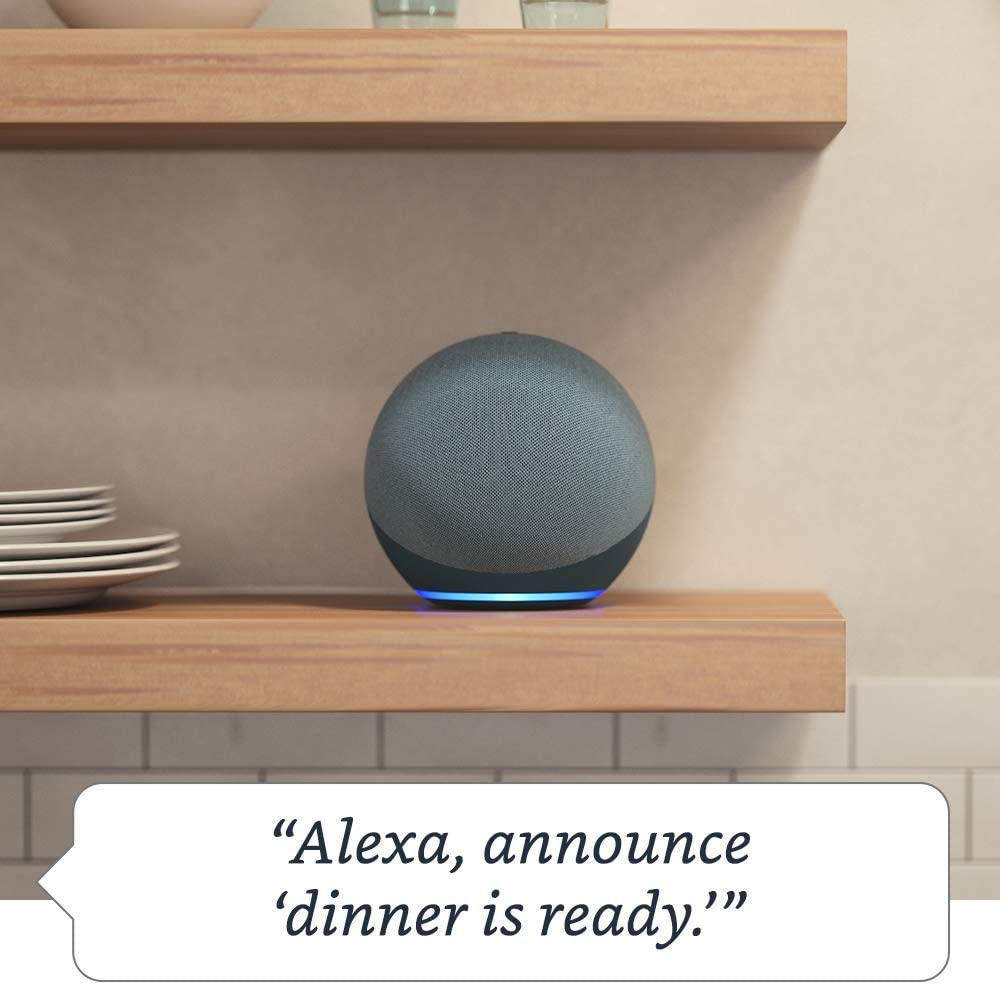
\includegraphics[width=0.4\textwidth]{./images/echodot4.jpg} % <- formatos PNG, JPG e PDF
	\caption[Amazon Echo 4th Generation smart speaker promotional material]{Amazon Echo 4th Gen Smart Speaker promotional material}
    \fonte{Amazon (2022)}
	\label{fig:echodot4}
\end{figure}

\begin{quote}
    \textit{This device is a gem! When I’m busy in the kitchen, for example, and can’t get
    to a computer to find info or music to play, Alexa would be there to listen
    and do what I ask.} \\
    Customer review from \cite{GaoPanWangChen2018}
\end{quote}

Alongside the devices themselves, entirely new markets have emerged such as the
third-party software extensions called \textit{Alexa Skills} \cite{Alexa2022}.

These skills function much like mobile phone apps, extending and enhancing the
functionality of the device and can be sold to end users.

Developers can then easily leverage the highly advanced machine learning models
-- which can be notoriously expensive to develop and maintain \cite{Phdata2021}
-- through Application Programming Interfaces (\sigla{API}{Application
Programming Interface}) and focus exclusively on their business logic.

\begin{figure}[htb!]
	\centering
	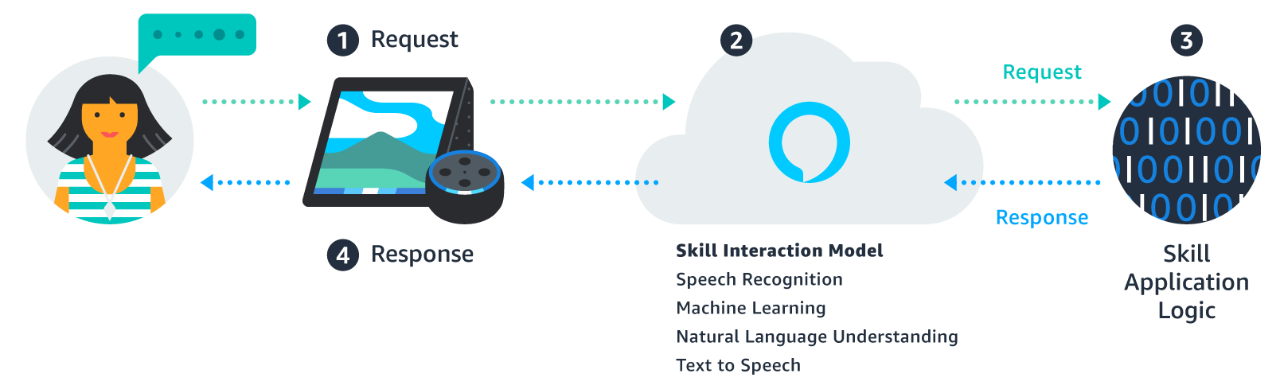
\includegraphics[width=0.9\textwidth]{./images/skills.png} % <- formatos PNG, JPG e PDF
	\caption[Diagram showing the steps of an interaction with an Alexa Skill]{Diagram showing the steps of an interaction with an Alexa Skill}
    \fonte{\cite{Alexa2022}}
	\label{fig:alexaskill}
\end{figure}

More impressively, such technological advancements have been able to reach a
considerable amount of households in a short period of time in developed
countries like the United States. 

\begin{figure}[H]
	\centering
	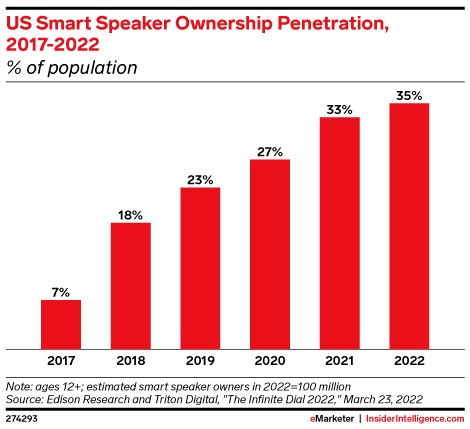
\includegraphics[width=0.6\textwidth]{./images/smartspeaker.png} % <- formatos PNG, JPG e PDF
	\caption[US Smart Speaker Penetration from 2017 to 2022]{US Smart Speaker Penetration from 2017 to 2022}
    \fonte{\cite{InsiderIntelligence2022}}
	\label{fig:smartspeaker}
\end{figure}

On developing countries such as Brazil, these innovations tend to
have delayed arrivals due to historical economic barriers but the potential
customer base has attracted big tech companies like Amazon, that are able
to shorten the arrival delay with their economic power.

\begin{figure}[h!]
	\centering
	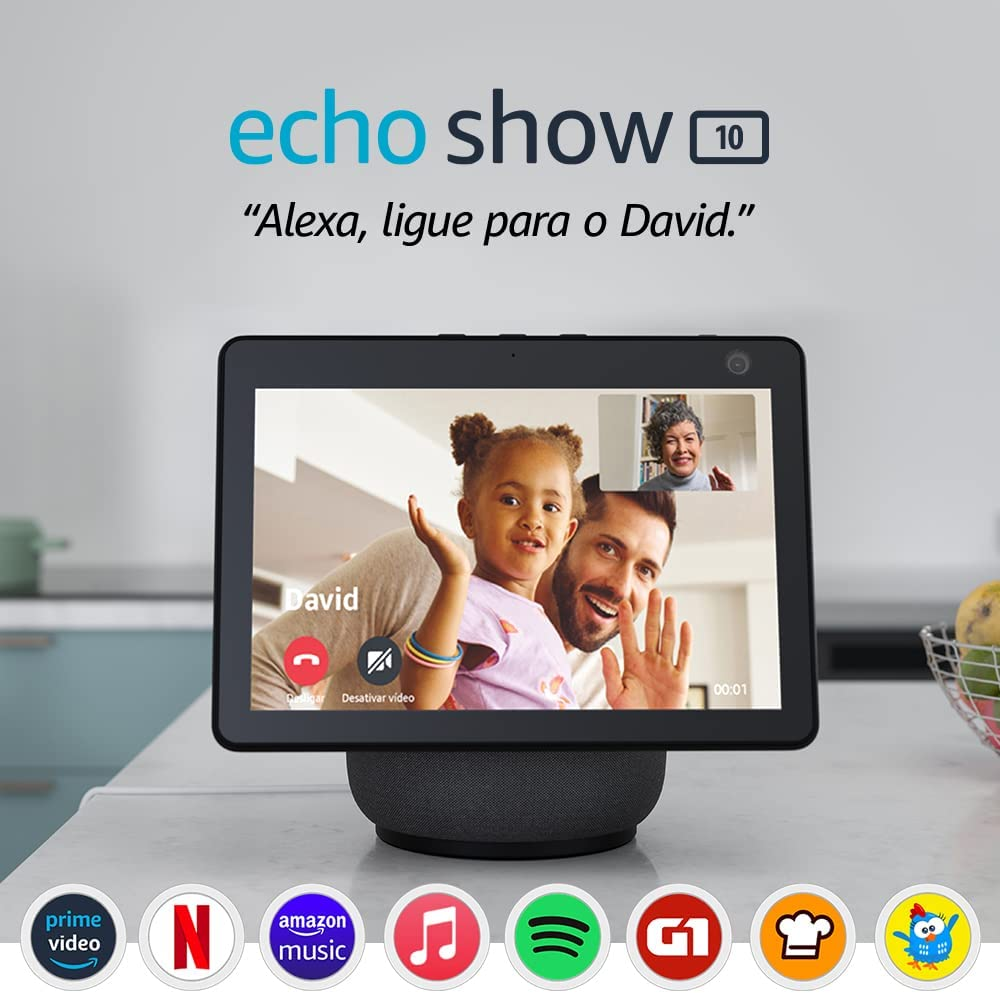
\includegraphics[width=0.4\textwidth]{./images/alexabr.jpg} % <- formatos PNG, JPG e PDF
	\caption[Localized promotional material for the Echo Show 10 targeting Brazilian customers]{Localized promotional material for the Echo Show 10 targeting Brazilian customers}
    \fonte{Amazon (2022)}
    \label{fig:alexabr}
\end{figure}

According to the research company IDC Brasil, the Brazilian home automation
market -- in which smart speakers are included -- would have reached US\$ 298
million on 2021, an impressive figure that might explain the attractiveness of
our market.

% Although these advancements might seem entirely beneficial at first, countless
% challenges have been found regarding privacy, ethical handling of personal
% customer data and overall negative experiences caused by increased
% dependencies, e.g what happens when you lose internet connection?
%
% These discussions are of the utter most importance given our current scenario
% and have been brought up by recent literature \cite{Echoes2022,He2019}
% but will be out of the scope of this work.


But even with all of these innovations impacting customer behaviors day by day, one
important aspect of consumer life still hasn't had any significant changes in
the last couple of years: \textbf{shopping on
physical stores}.

According to \sigla{ABRAS}{Associação Brasileira de Supermercados} - the
Brazilian Supermarket Association - the grocery retail sector has reached an
impressive total revenue of \textbf{R\$ 611 billion} in 2021 - roughly US\$ 117 billion on
October 2022 conversion rates - making up 7,03\% of the national \sigla{GDP}{Gross
Domestic Product}. About \textbf{28 million} customers visit one of the more than
\textbf{92.000} stores countrywide on a daily basis \cite{Abras2022}.

Despite all the technological advancement seen over the last few year and the
economic relevance of such sector, retail grocery shopping still exhibits the
same pain points found a decade ago. In a survey conducted in 2019, Capgemini
has found out five key pain problems related to physical stores in general
\cite{Capgemini2020}:

\begin{enumerate}
        \item Long queues for payment checkout
        \item Out of stock products
        \item Difficulties in locating products in the store
        \item Not being able to find a store associate to help
        \item Lack of product information when I select products
\end{enumerate}

\begin{figure}[H]
	\centering
	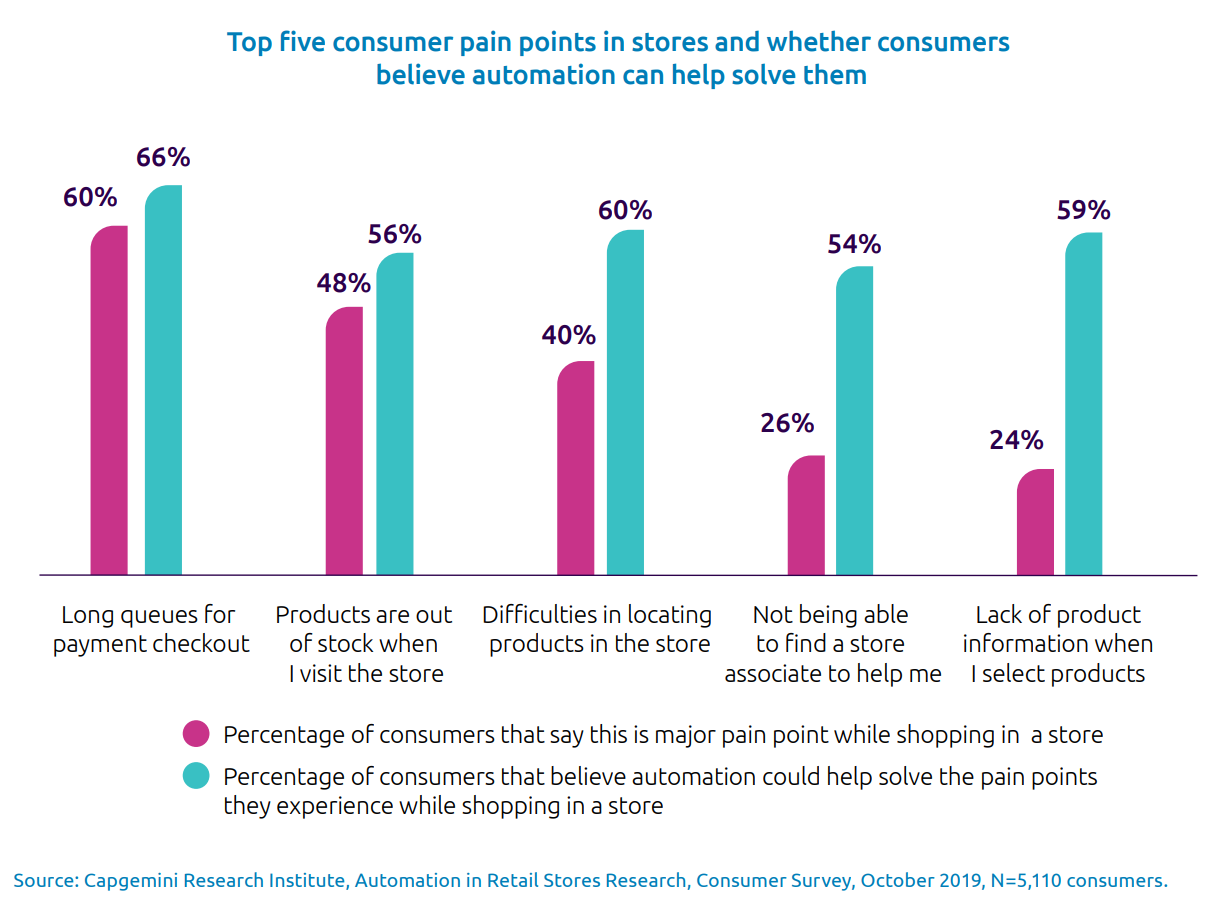
\includegraphics[width=0.8\textwidth]{./images/painpoints.png}
    \caption[Top five customer pain points in retail stores]{Top five customer pain points in retail stores}
    \fonte{\cite{Capgemini2020}}
    \label{fig:capgemini}
\end{figure}

More interestingly, the survey points out that at least half of the survey
respondents believe that all of the five pain points can be solved through
\textbf{automation}. Even in light of the recent pandemic scenario, innovations
that increase automation such as e-commerce platforms had their adoption
increased in 2020 but 2021 showed a trend of consumers shifting
back to their pre-pandemic behavior, favoring physical retail stores
\cite{Kantar2022}.

It is in this scenario of customer pain and enormous market potential that this
thesis will explore a technological solution to improve customer experience and increase sales,
namely the \textbf{smart shopping cart}.

\section{Current scenario}

In this next section, we'll explore some of the existing solutions and the user experience
provided by them.

\subsection{Caper Cart}

Developed by the Caper\footnote{https://caper.ai} company, the Caper Cart was the worlds's first AI-powered smart cart \cite{Caper2020}

The first version was launched in 2017 and offered grocers the
great advantage of not requiring any infrastructure overhaul for deployment.

\begin{figure}[H]
	\centering
	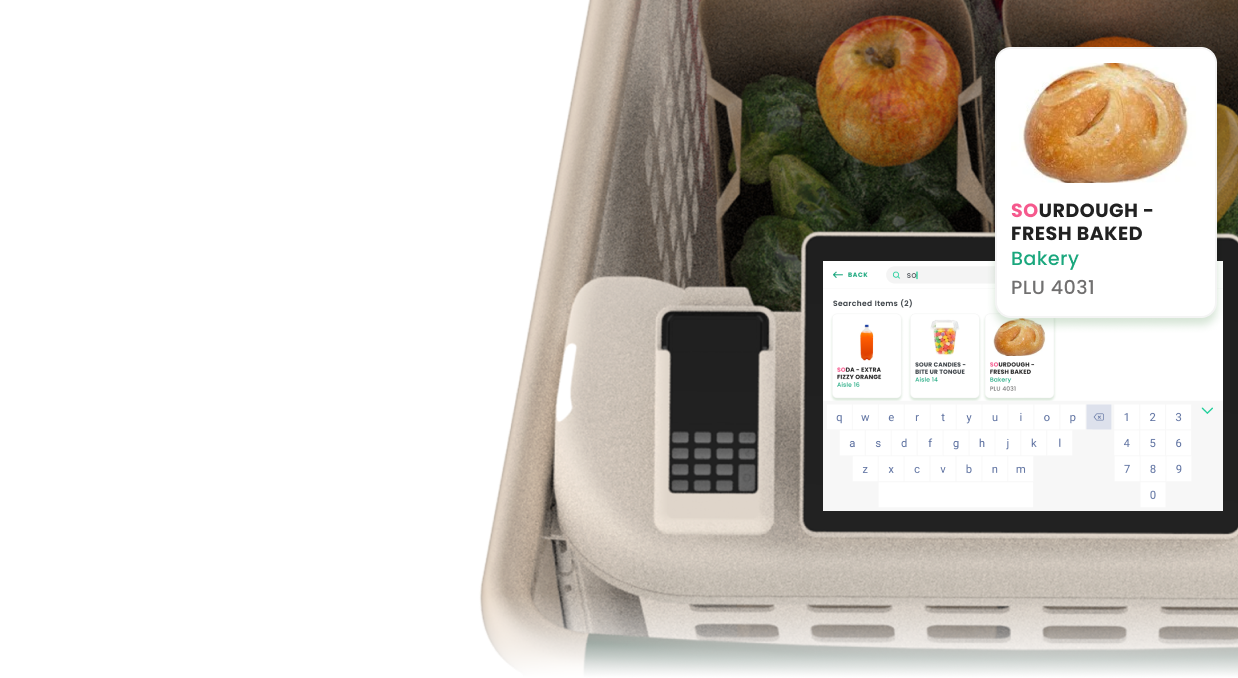
\includegraphics[width=0.7\textwidth]{./images/capercartui.png}
	\caption[Caper Cart user interface]{Caper Cart user interface}
    \fonte{Caper (2020)}
	\label{fig:caperui}
\end{figure}

\begin{figure}[H]
	\centering
	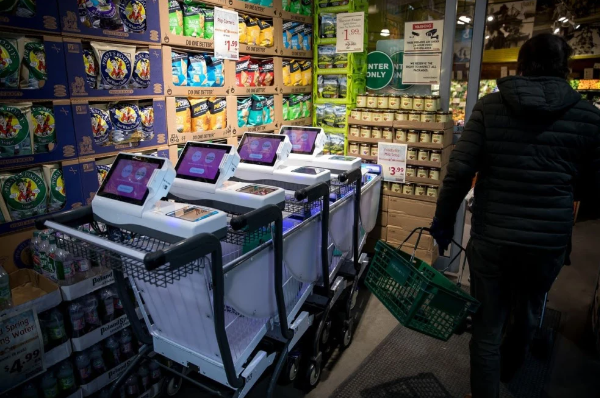
\includegraphics[width=0.7\textwidth]{./images/caper.png}
	\caption[Caper Cart at a retail store]{Caper Cart at a retail store}
    \fonte{Caper (2020)}
	\label{fig:caperatretail}
\end{figure}

For end users, it offered visual product recognition and a payment terminal,
allowing them to avoid the dreaded queues by the end of their shopping session.
Additionally, customers were able to search products, get discounts and locate
items more easily with the help of the interactive user interface provided by the cart.

Although Caper does not publicize the cost of each cart, it is estimated that each unit costs between
\textbf{US\$ 5,000 and 10,000} \cite{TWP2021}.

Acquired by Instacart\footnote{https://instacart.com} in 2021 for US\$ 350 million, Caper is developing in 2022 the 
third version of its Smart Shopping Cart, advertising an increase of \textbf{65\% in the basket
volume} and a \textbf{10 month} break even period.

\begin{figure}[H]
	\centering
	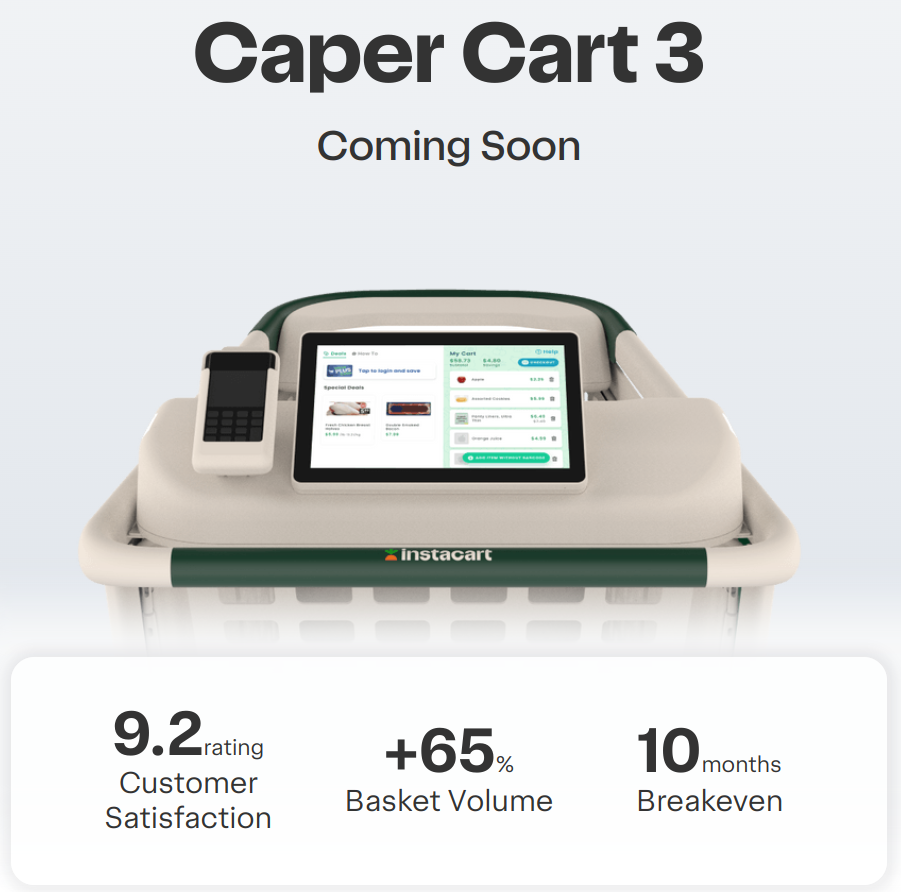
\includegraphics[width=0.7\textwidth]{./images/capercart3.png}
	\caption[Caper Cart 3 promotional material]{Caper Cart 3 promotional material}
    \fonte{Caper (2022)}
	\label{fig:nextop}
\end{figure}


\subsection{Amazon Dash Cart}

Available at the Amazon Fresh\footnote{https://www.amazon.com/fmc/m/30003175?almBrandId=QW1hem9uIEZyZXNo} retail chain, the
Amazon Dash Cart is the company's first smart cart available to end users.

According to Amazon, it uses computer vision and sensors to allow customers to
simply add items to their cart like they usually would. The cart accounts all
the items present in the cart, displaying a list which includes their prices
and subtotal. By the end of their item selection, customers can check-out
automatically without having to go through queues, solving the biggest customer
pain point pointed out by \cite{Capgemini2020}.

\begin{quote}
\textit{Looking to make grocery trips quicker? With the Amazon Dash Cart you can skip the checkout line and roll out to your car when you are done.}

\textit{The Dash cart uses a combination of computer vision algorithms and sensor fusion to help identify items placed in the cart - simply grab an item, scan it on one of the Dash Cart cameras, and place it in the cart like you normally would.}
\\
Amazon (2022)
\end{quote}

\begin{figure}[H]
	\centering
	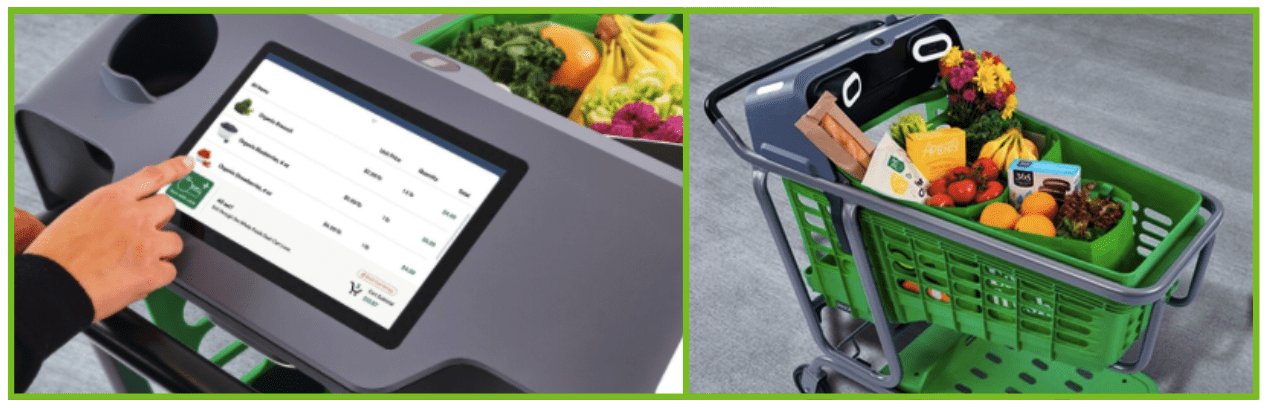
\includegraphics[width=0.8\textwidth]{./images/dashcart.png}
    \caption[Amazon Dash Cart]{Amazon Dash Cart}
    \fonte{Amazon (2022)}
    \label{fig:dashcart}
\end{figure}

In addition to the item accounting capabilities, the user interface provided by
the Cart also allows customers to search for the location of items  in the
store and see more information about them, improving the customer experience.

One of its quirks is that it requires the download and usage of an mobile phone
app for using the cart, something not required by Caper's Cart.

As of October 2022, the Amazon Dash Cart is exclusively available at the Amazon
Fresh chain and therefore no commercial information regarding cost per unit is
available.

\subsection{Nextop}

Founded in 1997, Nextop\footnote{https://nextop.com.br} is a Brazilian company
that develops products with a focus on the grocer market with an emphasis on
loss prevention.

According to the company, the Smart Cart Nextop is the first smart cart
deployed in Brazil and Latin America and was initially rolled out to the Enxuto
supermarket chain in 2022 \cite{Paraiba2022}.

\begin{figure}[H]
	\centering
	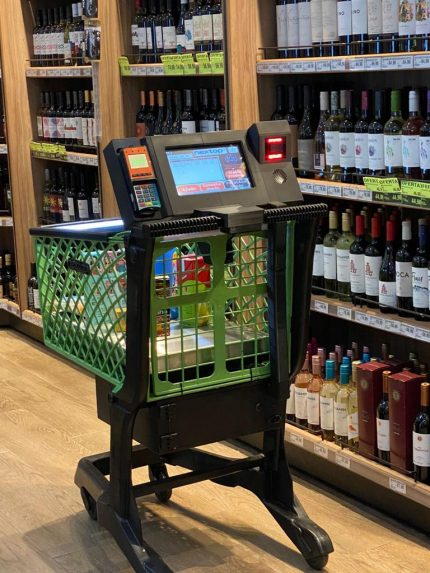
\includegraphics[width=0.4\textwidth]{./images/nextop.jpeg}
	\caption[Smart Cart Nextop® deployed to a Brazilian supermarket]{Smart Cart Nextop® deployed to a Brazilian supermarket}
    \fonte{Nextop (2022)}
	\label{fig:nextop}
\end{figure}

In contrast to the carts developed by Amazon and Caper, Nextop's cart
requires customers to first scan the product using the integrated bar code
reader, as shown on Figure \ref{fig:nextopui}. This way, the product advertises for a
\textit{triple validation} system, using the cameras, sensors and the barcode scanner 
to prevent losses \cite{Nextop2022}.

\begin{figure}[H]
	\centering
	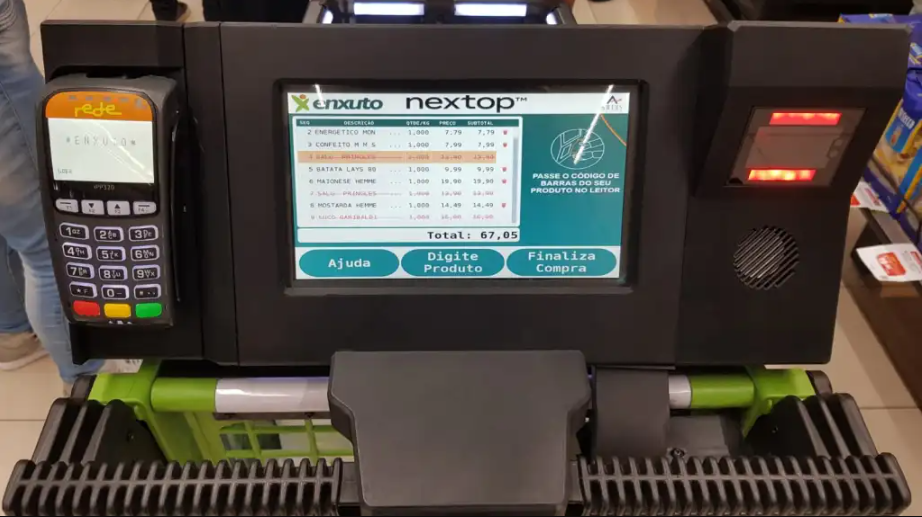
\includegraphics[width=0.9\textwidth]{./images/nextop2.png}
    \caption[Smart Cart Nextop® user interface with a payment terminal]{Smart Cart Nextop® user interface with a payment terminal}
    \fonte{\cite{Paraiba2022}}
	\label{fig:nextopui}
\end{figure}

Although loss prevention is an important selling point in the Brazilian market,
the usage of the barcode scanner creates, in our opinion, a worse end customer
experience, becoming a \textit{mobile checkout station}. Also, the product does not
include additional features such as product location search and item details. 

\begin{figure}[H]
	\centering
	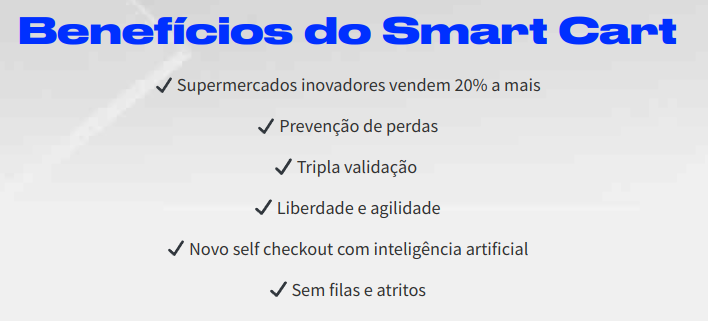
\includegraphics[width=0.9\textwidth]{./images/nextoppromo.png}
    \caption[Smart Cart Nextop® promotional material targetting supermarket owners]{Smart Cart Nextop® promotinal material targetting supermarket owners. It advertises for improved sales, loss prevention and reduced queues.}
    \fonte{\cite{Nextop2022}}
	\label{fig:nextopui}
\end{figure}

Offering a solution to the main end user pain point of having to go through
long queues, the product also advertises increased sales as a result of the
innovative approach and also allows a deeper understanding of the customer
journey by collecting analytical data \cite{Paraiba2022}.

\begin{quote}
\textit{We are offering our customers an innovative and unique shopping experience within Enxuto}

\textit{With the smart cart, we broke through this barrier and managed to monitor the
entire customer's purchase circuit in the physical store. We have moved
from the identified ticket era to the end-to-end identified journey}

    Bruno Bragancini Junior, \sigla{CEO}{Chief Executive Officer} of the Enxuto Group \cite{Paraiba2022}
\end{quote}

According to Nextop's CEO, Juliano Camargo, the company has already invested \textbf{R\$ 8.5 million} - about US\$ 1.63 million on October 2022 - and \textbf{4 and half years}
of research and development.

Each Smart Cart is estimated to cost around \textbf{R\$ 120,000  or around US\$ 23,020} on October 2022 \cite{Paraiba2022}.

\section{Objectives}

After presenting the problem domain and the current market scenario, in this section we discuss the 
objectives of this work.

\subsection{Main objective}
Develop a prototype of a smart shopping cart that utilizes computer
vision and sensor data for product recognition.

\subsection{Granular objectives}
\begin{itemize}
    \item Build a mechanical assembly for the prototype
    \item Develop an interactive user interface for the prototype
    \item Collect a product dataset for training a deep learning model
    \item Train a Deep Learning model capable of detecting target products
	\item Learn the practical challenges of developing a Deep Learning based product
    \item Understand the economic viability of such a project in the Brazilian context
\end{itemize}

\chapter{Theoretical Background}

In this section, we'll define in greater detail the theory behind some most
relevant techniques used in the development of the prototype.

This section can be skipped for readers with familiarity on the topics discussed.

\section{Neural Networks}

Neural Networks, or Artificial Neural Networks (\sigla{ANN}{Artificial Neural Network}),
are networks built out of interconnected decisional Neurons that aim to replicate 
the behaviour of the human brain, enabling computational systems to cluster data
and to make predictions \cite{IBMNeuralNetworks}. 

A Neuron is similar to a Digital Logic Gate, which is capable of producing 
different outputs depending on the input signals that are sent to it.
A Neuron has weights, which are the coefficients that are used for calculating
the outputs; and biases, which are the boundaries that represent how prone is an output
to fit into a specific category of output. 

The main difference between a digital logic gate and a Neuron is that, because neurons are
parameterized with weights and biases, we can apply \textit{learning algorithms}
to tune (or train) Networks of Neurons using real world or synthetic data \cite{Nielsen2015}.

\subsection{Neurons}

One of the most popular types of Neurons is the Perceptron, introduced by 
\cite{Rosenblatt1958}. 
A perceptron takes one or more binary inputs and produces a single binary output.

\begin{figure}[H]
	\centering
	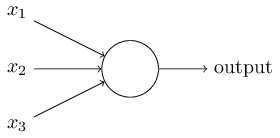
\includegraphics[width=0.5\textwidth]{./images/perceptron.png}
	\caption[The Perceptron Neuron]{The Perceptron Neuron}
    \fonte{\cite{Nielsen2015}}
	\label{fig:perceptron}
\end{figure}

A Neuron does not necessarily have binary inputs and outputs. In fact, 
contemporary systems commonly use a different type of Neuron known as the Sigmoid Neuron, 
which take real numbers as inputs and also produces continuous outputs 
within the boundaries of the sigmoid curve instead of discrete zeroes and ones. 
This is particularly useful for learning, since in Perceptrons small differences in the 
weights or biases could yield to different outputs without a full transparency 
on how close the output would have been to a different one \cite{Nielsen2015}.

\begin{figure}[H]
	\centering
	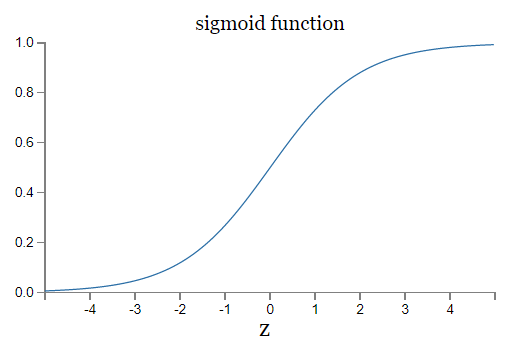
\includegraphics[width=0.5\textwidth]{./images/sigmoid-function.png}
	\caption[Sigmoid Function]{Sigmoid Function}
    \fonte{\cite{Nielsen2015}}
	\label{fig:sigmoid}
\end{figure}

\subsection{Learning Algorithms}

There are three main types of learning algorithms: Supervised, Unsupervised and Reinforcement.
Supervised learning is employed when you know what are your expected outputs and use this
information to feed (train) your models such that they can start doing that on their own; 
Unsupervised learning is applied when you do not know what are the expected labels 
in your data or you do not have them available; and Reinforcement learning is used when
algorithms need to replicate specific behaviors depending on the feedback that is
provided to them \cite{CourseraML}. 

Supervised learning is typically employed for regression and classification tasks; 
Unsupervised Learning is typically used for clustering raw data into different buckets
without necessarily knowing how to do it or having the labelled data available;
and Reinforcement learning is often applied in control systems.
This work will primarily focus on Supervised Learning, since our proposed project uses
Object Detection and is trained based on labelled data samples.

As for the learning algorithms used for training Neural Networks, 
the standard algorithm is the Stochastic Gradient Descent (\sigla{SGD}{Stochastic Gradient Descent}).
Alike other gradient descent algorithms, the SGD aims to minimize the loss function of a given
Neural Network iteratively. In simple terms, it consists of an iterative optimization algorithm defined by an
objective function to minimize the error.

The key feature of the SGD is that it does that very efficiently by initializing the weights
and biases randomly and then fine tuning it during training by trying to find the higher descents 
(or the higher derivatives of the error function), reducing the number of necessary iterations, 
which is particularly important considering that the amount of data that is used to train AI
models has increased considerably over the last few years \cite{CornellSGD}.

Finally, in terms of the way how the SGD is computed in Neural Networks, a widely adopted approach 
for Supervised Learning is Backpropagation. Backpropagation computes the gradients of the final 
layers of a Neural Network first, and the gradients of the first layers at last, 
and it reuses partial computations of the gradient from a layer to the other to compute each layer's 
gradient, making it more efficient than calculating each layer's gradient separately \cite{BrilliantBackpropagation}. 

\section{Deep Learning}

Deep Learning defines a group of AI algorithms that use advanced learning techniques on the 
top of ANNs to train models that allow systems to forecast and clusterize data 
efficiently \cite{IBMDeepLearning}.
Deep Learning algorithms use Neural Networks that have three types of layers:
Input Layer, Hidden Layer and Output Layer.
        
\begin{figure}[H]
	\centering
	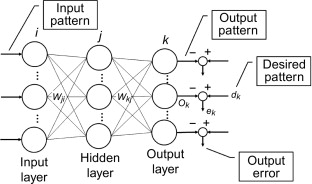
\includegraphics[width=0.6\textwidth]{./images/three-layered-ann.jpg}
	\caption[Three Layered Neural Network]{Three Layered Neural Network}
    \fonte{\cite{ARAKI2015121}}
	\label{fig:threeLayeredAnn}
\end{figure}

The Input Layer takes the input data that will be fed into the model for training,
$x_i$, and produces the weighting coefficients $w_{ji}$. Input Layers
typically have the role of encoding the input data into a structure that can be processed by the 
subsequent hidden layers \cite{Paranjape2020}.

The $w_{ji}$ coefficients are then used to feed the Hidden Layer of the network,
which produces the weighting coefficients $w_{kj}$. The Hidden Layers of a Deep Learning 
Neural Network are used for the heavy processing of the encoded input data by applying a series of 
mathematical operations that ultimately makes it possible to break down the most important features
of the data and to produce comprehensive outputs to the decisional layers of the network
\cite{DeepAI_HiddenLayer}.

\subsection{Transfer Learning}

Another key technique applied by developers when training Deep Learning models is
\textit{Transfer Learning}. 
It consists of reusing pre-trained networks, which were tuned in other datasets -- usually big and
somehow related to the one that you are going to run your inferences on -- for training custom models.

Transfer Learning works by freezing the weights and biases present in specific layers of a
pre-trained Network -- usually being the hidden layers, which are the feature extractors -- 
when training customized models. This way,  only some layers of the Network -- usually the last layers, which 
are the deciders -- effectively have to be tuned.

The biggest advantages of Transfer Learning are that, because it allows for
training only specific layers of an architecture to get a custom model, the
training process is much faster than it would be if the whole network had to be
retrained; and additionally less training data is required for achieving a good
performing model, since you reuse the work done on the previous training
\cite{CS231N}.

\section{Tensor Processing Unit}
\label{sec:TPU}

With the increased adoption of DNNs in various workloads and their specialized
and heavy compute nature, Google started the development of a domain specific
architecture (\sigla{DSA}{Domain Specific Architecture}) which resulted in a
first generation custom chip, named Tensor Processing Unit (\sigla{TPU}{Tensor
Processing Unit}), deployed to their data centers since 2015 \cite{Google2015}.
The developed TPU had the target of improving the inference phase of DNNs and
achieved a performance improvement of \textbf{15-30 times} when compared to
contemporary hardware of paired or reduced power consumption.

\begin{figure}[H]
	\centering
	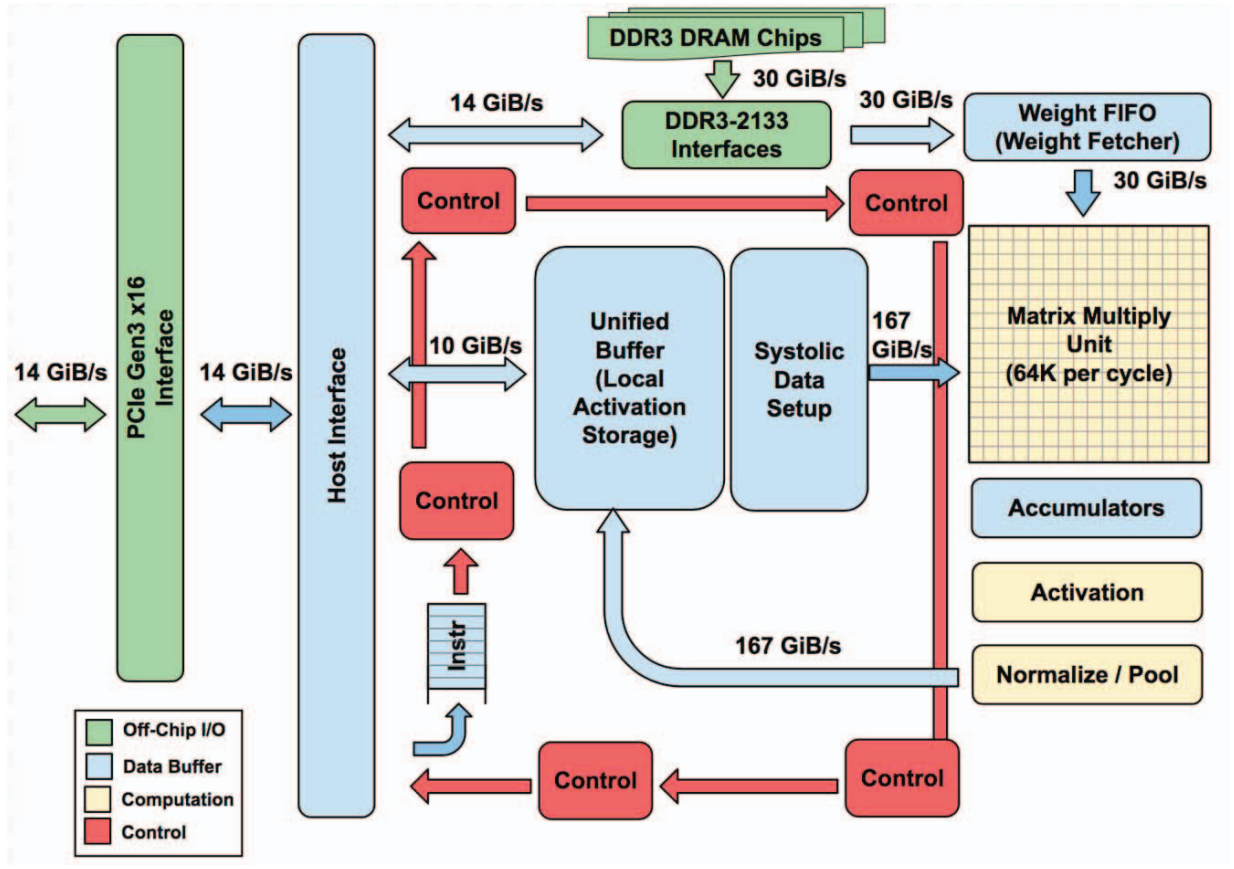
\includegraphics[width=0.6\textwidth]{./images/tpublock.png}
	\caption[TPU block diagram]{TPU block diagram. The main computation, matrix multiplication, is done by the yellow units.}
    \fonte{\cite{Google2015}}
	\label{fig:gauge1}
\end{figure}

Since the first generation TPU described in a 2018 paper \cite{Google2015},
Google has released the TPU into commercials products made available to third
parties. Most notably, the Google Coral\footnote{https://coral.ai} initiative
offers ready-to-use development boards that embedded TPU chips, allowing
developers to leverage the improved DNN performance in their applications.

\begin{figure}[H]
	\centering
	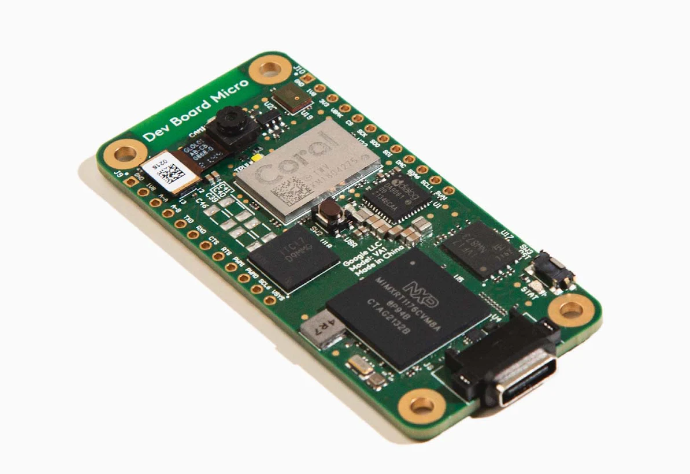
\includegraphics[width=0.5\textwidth]{./images/coralboard.png}
	\caption[Coral Dev Board Micro]{Coral Dev Board Micro. It includes a microphone, camera and the Coral Edge TPU in a single board package.}
    \fonte{Coral.ai}
\end{figure}

\section{Strain Gauge}

For measuring weight, one of the most common transducers used is the strain
gauge. A strain gauge is a device whose measured electrical
resistance varies with changes in its applied force, as a consequence of the
mechanical deformation \cite{Stefanescu}.

\begin{figure}[H]
	\centering
	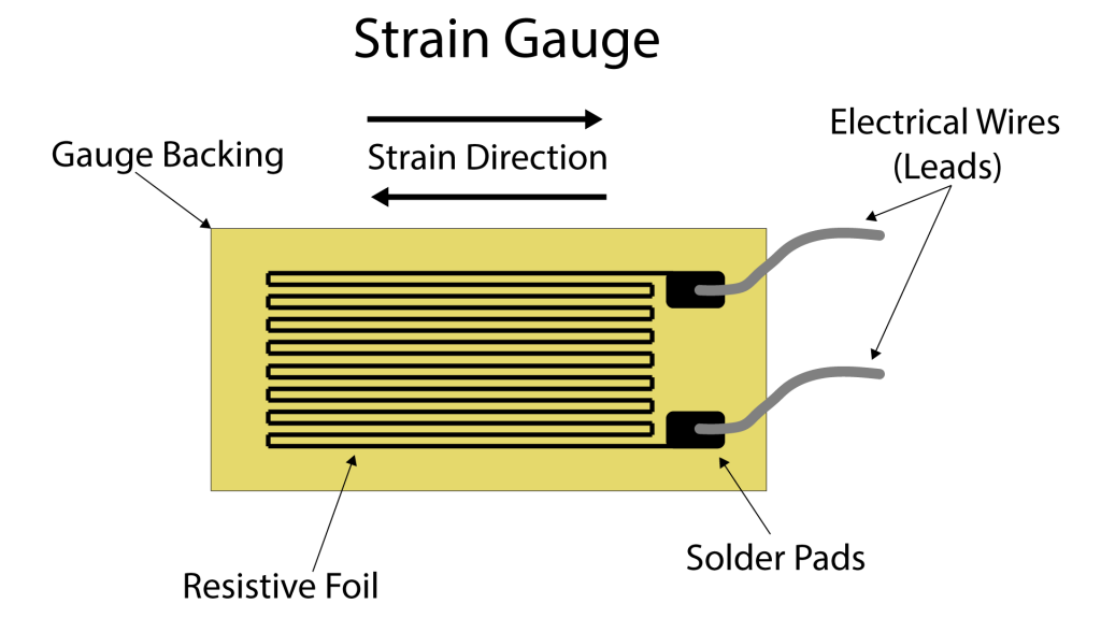
\includegraphics[width=0.5\textwidth]{./images/straingauge.png}
	\caption[Typical Strain Gauge construction]{Typical Strain Gauge construction}
    \fonte{\cite{Michigan2020}}
	\label{fig:gauge1}
\end{figure}

In practice, however, the resistance variations observed after applying a
mechanical strain are minute and can be difficult to measure. To solve that issue,
and to also provide a signal which can be later used as the input of an
Analog-to-Digital Converter (\sigla{ADC}{Analog-to-Digital Converter}), the Wheatstone
Bridge circuit can be used \cite{Michigan2020}.

\begin{figure}[H]
	\centering
	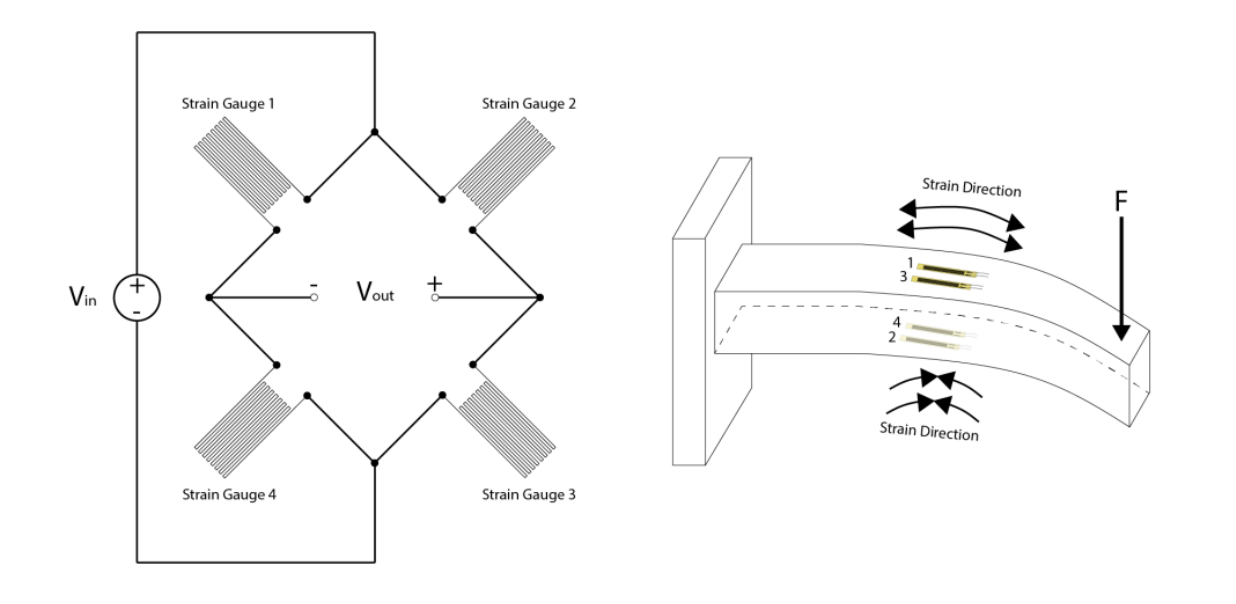
\includegraphics[width=0.9\textwidth]{./images/straingauge2.png}
	\caption[Wheatstone Bridge circuit using four strain gauges]{Wheatstone Bridge circuit using four strain gauges}
    \fonte{\cite{Michigan2020}}
	\label{fig:gauge2}
\end{figure}

When no load is applied, the bridge is balanced and the output voltage
$V_{out}$ should be zero. If any strain is applied to the gauges, the bridge
will become unbalanced, and therefore will result in a non-zero output voltage.
Since the voltage variation tends to be small, in the order of millivolts, signal amplification is usually
required for pairing the bridge with commercially available ADCs \cite{HorowitzHill2015}.

It can be shown that the relation between $V_{out}$ and $V_{in}$, $S$, shown on Figure \ref{fig:gauge2}, can be
calculated as \cite{Stefanescu}:

\begin{equation}
    \label{eq:strain}
    S = \frac{V_{out}}{V_{in}} = k\frac{\Delta l}{l}
\end{equation}
where $k$ is known as the \textit{gauge factor}, related to the physical
construction and materials of the strain gauge, and $\frac{\Delta l}{l}$ is the
relative variation of length or strain.

With that, Equation \ref{eq:strain} indicates that the output voltage $V_{out}$
will be linearly proportional to the amount of strain applied, providing the
desired sensing capability.

\section{Load Cell}

Using strain gauges directly can be difficult since a proper
mechanical structure and arrangement is crucial for the sensors to function
properly. For that, commercially available \textit{Load Cells} offer ready to
use mechanical packages that embed the strain gauges for weight sensing
using electronic circuits.

In general, they consist of a spring element onto which the gauges are placed.
When load is applied to the cell, the strain gauges will be stressed and
therefore provide the desired sensing \cite{HBM2022}.

\begin{figure}[H]
	\centering
	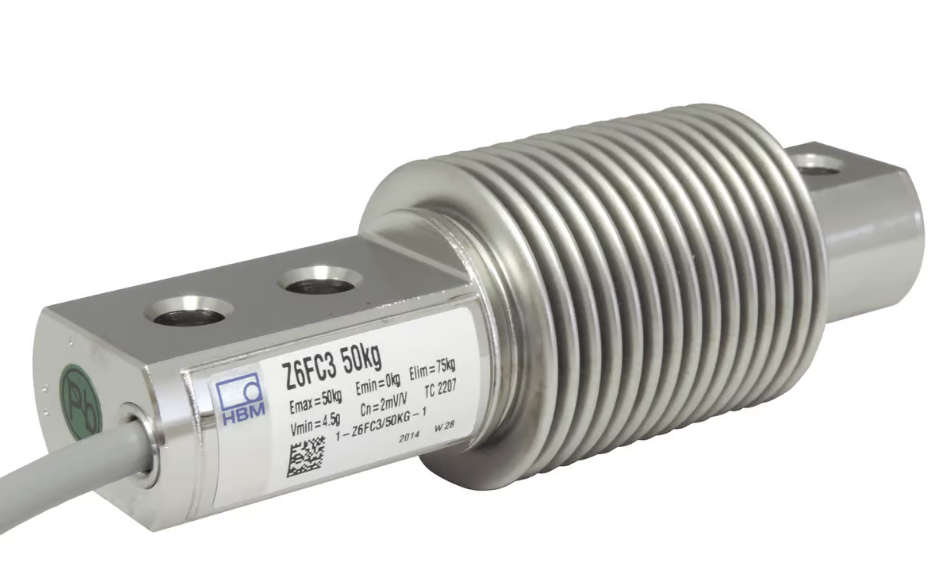
\includegraphics[width=0.3\textwidth]{./images/hbmz6.png}
	\caption[HBM Z6 commercial load cell]{HBM Z6 commercial load cell}
    \fonte{HBM}
	\label{fig:gauge2}
\end{figure}

\chapter{Development}
\label{chap:desenv}

In this section, we describe the development of the \textit{zCart} smart cart
prototype. All the source code related to the prototype is available at a
GitHub repository\footnote{https://github.com/fsmiamoto/zcart}

\section{Design}
\label{sec:design}

As a first step in developing our prototype, a set of
high level goals was defined to guide the initial design:

\begin{enumerate}
    \item Handle user interactions and give visual feedback
    \item Store the current set of products present in the cart and their respective information
    \item Recognize the addition or removal of products, including quantities.
\end{enumerate}

With those goals in mind, the high level architecture of the prototype
was designed and is shown in Figure \ref{fig:architecture}.

For each goal, a dedicated software application will be used and those
applications will communicate using \sigla{TCP}{Transmission Control Protocol}
network sockets \cite{Kurose2013} with industry standard application protocols such as
\sigla{HTTP}{Hypertext Transfer Protocol}\footnote{First defined in
\sigla{RFC}{Request For Comments} 1945} and WebSocket\footnote{Defined in RFC 6455}.
Most of the HTTP communication will follow the widespread REST pattern \cite{Roy2000}.

For handling the first goal, the \textit{User App} will request data
from other applications and will display the information to end users and allow
them to interact with the cart using a touch enabled LCD display. 

The \textit{Cart Service} will be in charge of the second goal,
handling requests from the \textit{User App} that request data or incur in any
side effects, such as completing a purchase. The \textit{Cart Service} uses a
\textbf{relational database} \cite{Silberschatz2010} as its primary database. Namely
\textbf{SQLite}, considered to be the world's most deployed database due to its
massive adoption in mobile
devices\footnote{https://www.sqlite.org/mostdeployed.html}. The simplicity of
SQLite -- the entire database is contained within a single file -- great
library support in common programming languages and the use of the familiar
relational modeling, including \sigla{SQL}{Structured Query Language}
\cite{Nield2016}, were key factors in choosing it.

In order to provide real time updates to the \textit{User App}, the Cart Service has a
WebSocket API endpoint that allows the User App to listen to updates such as a product addition
and then display a notification to the end user.

For the third goal, the \textit{Product Recognizer} application will be responsible
for processing a camera feed and weight sensor data to be able to tell if any products
were added of removed from the cart. Any detected changes will be communicated to the
Cart Service, which will be responsible for persisting those changes on the database. 

All three applications will executed under a Linux \cite{Tanenbaum2015} 
based environment on a Raspberry Pi\footnote{https://www.raspberrypi.com} 4 Single Board
Computer (\sigla{SBC}{Single Board Computer}) - a complete computer built on a single 
circuit board with a microprocessor, memory and input/output devices.

The advantages of using a Linux environment for the development are many, but
being able to leverage its concurrency capabilities, having built-in drivers
for readily available hardware and leveraging open source projects are some 
worth mentioning.

\begin{figure}[H]
	\centering
	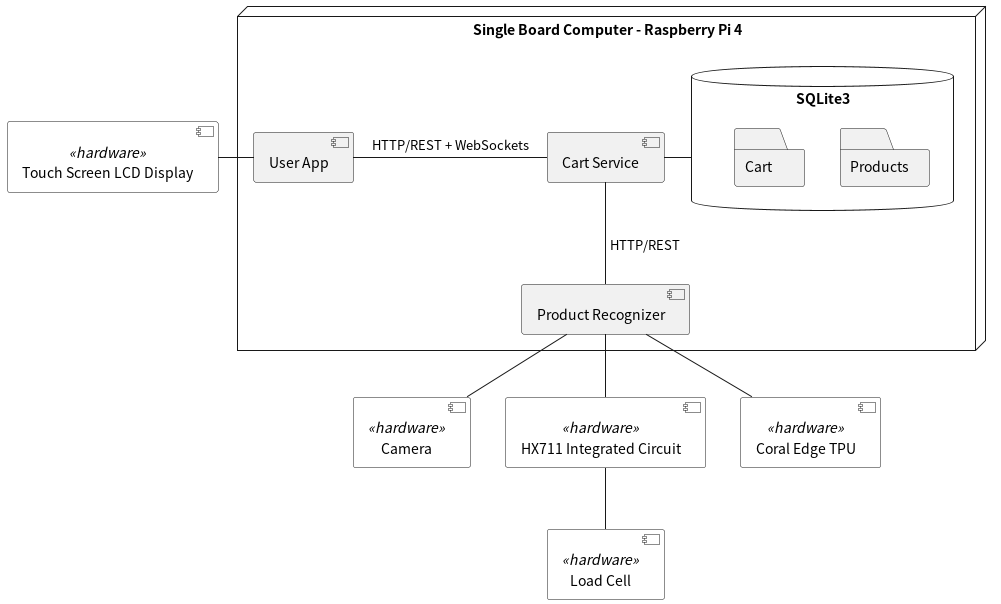
\includegraphics[width=1\textwidth]{./images/zCart.png}
	\caption[High level architecture of zCart]{High level architecture of zCart}
	\fonte{Own work}
	\label{fig:architecture}
\end{figure}

\begin{figure}[H]
	\centering
	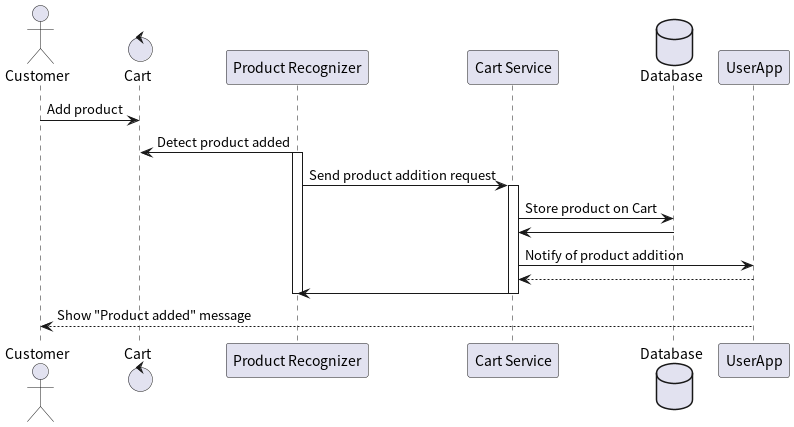
\includegraphics[width=1\textwidth]{./images/E2E.png}
	\caption[End-to-end sequence diagram for a product addition]{End-to-end sequence diagram for a product addition}
	\fonte{Own work}
	\label{fig:e2eseq}
\end{figure}

\subsection{Architectural Guidelines}
In creating the zCart architecture, the following guidelines were followed:

\begin{itemize}
    \item Create a separate software application for each goal domain
    \item Use well defined standards for communication between applications.
    \item All databases should be owned by a single application. 
    \item Any interaction that requires an update to a given database that is
        not owned by an application should be done through an API and not
        directly on the database.
    \item Decouple the user interface from how the data displayed is stored and transmitted
\end{itemize}

These guideline are based on known best practices from the software 
development industry including API-first design and segregation of
responsibilities \cite{Sam2021,Kong2022}, which are key for future architectural
evolution.

In the next sections, each application will be  detailed.

\section{User App}

For developing the User App, we have used web technologies such 
as HTML, CSS \cite{Duckett2011} and JavaScript \cite{Flanagan2020} through the 
React\footnote{htps://reactjs.org} framework. 

Using web-based technologies allows the User App to be displayed on any 
device capable of running a web browser; and having mature tooling for 
development, testing and debugging are important factors that influenced 
our decision.

As an alternative, developing Linux native graphical applications through
toolkits such as GTK\footnote{https://gtk.org} and Qt\footnote{https://qt.io}
might have yielded better performance but our unfamiliarity with those would be
a challenge.

\begin{figure}[H]
	\centering
	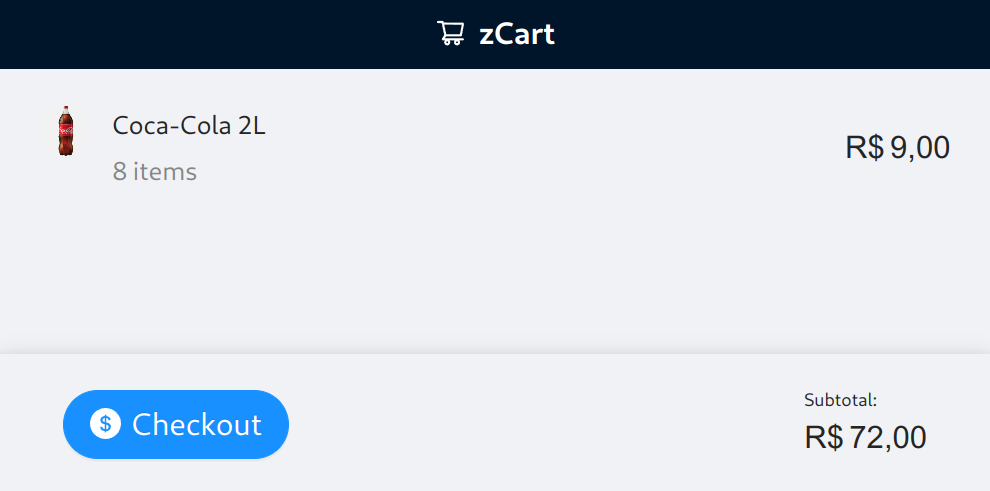
\includegraphics[width=0.8\textwidth]{./images/ui.png}
	\caption[User App Interface display a single product]{User App Interface displaying a single product}
	\fonte{Own work}
	\label{fig:userapp}
\end{figure}

As shown on Figure \ref{fig:userapp}, the main objective of the User App is to
provide a visual feedback mechanism for end users of the zCart.

It displays the current products added to the cart, their amounts and also the
price for each item. The subtotal price for all products added to the cart is
calculated and also displayed on the interface. Notifications are also
displayed when the user adds or removes a product from the cart. Finally, the
User App provides a \textit{Checkout} button to simulate the payment process
and act as a Proof-of-Concept (\sigla{PoC}{Proof-of-Concept}), because a functional
implementation of a payment mechanism is out of scope for our prototype.

More screenshots showing the user experience are available in Appendix \ref{ap:userapp}.

\begin{figure}[H]
	\centering
	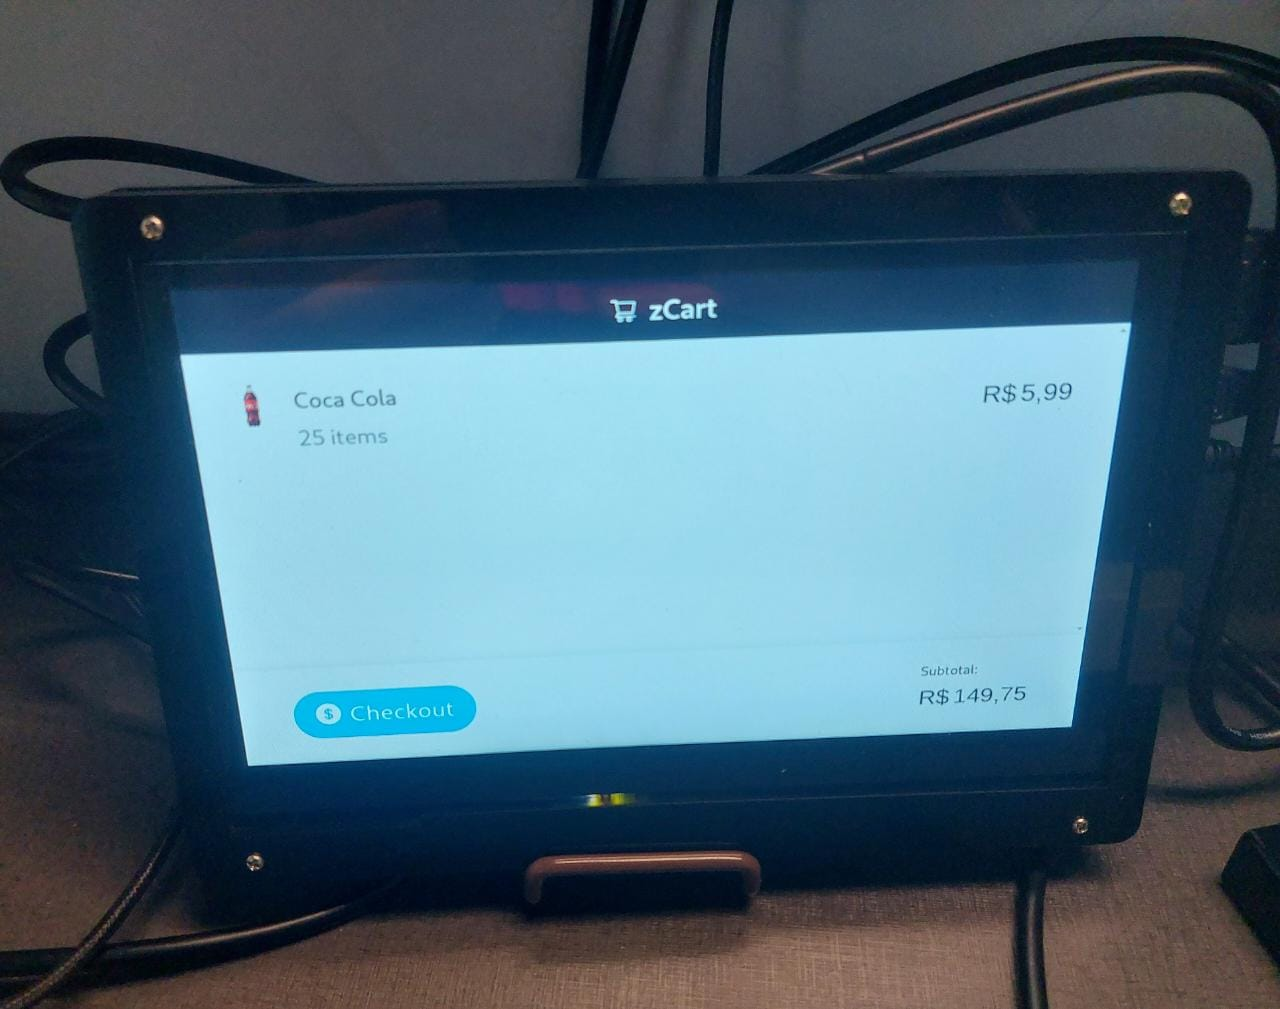
\includegraphics[width=0.6\textwidth]{./images/lcddisplay.jpeg}
	\caption[LCD Display showing the User App during development]{LCD Display showing the User App during development}
	\fonte{Own work}
	\label{fig:dummy}
\end{figure}

In terms of the data flow, the User App requests all data from the Cart Service, which exposes API endpoints for
getting the list of products of a given cart, establishing a WebSocket connection for notifications and performing
the PoC checkout.

\begin{figure}[H]
	\centering
	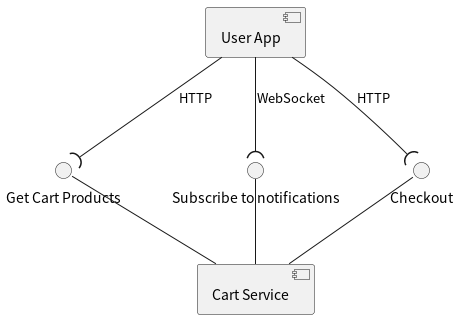
\includegraphics[width=0.6\textwidth]{./images/diagrams/UserApp.png}
	\caption[User App and Cart Service interactions]{User App and Cart Service interactions}
	\fonte{Own work}
	\label{fig:dummy}
\end{figure}

\section{Cart Service}

As described in Section \ref{sec:design}, the Cart Service will act as a
centralized \textit{source of truth}, storing the overall \textbf{state} of the
cart.

For that, it will responsible for managing the SQLite database and exposing API
endpoints for the required state changes e.g. adding a product.

\begin{figure}[H]
	\centering
	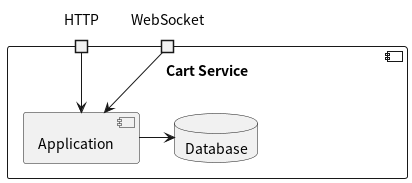
\includegraphics[width=0.6\textwidth]{./images/diagrams/CartService.png}
    \caption[Cart Service architecture]{Cart Service architecture. The database
    is contained withing the Cart Service boundary and it is not exposed in the
    public APIs}
	\fonte{Own work}
	\label{fig:dummy}
\end{figure}

For the HTTP endpoints, the application uses the REST \cite{Roy2000} pattern
with JavaScript Object Notation (\sigla{JSON}{JavaScript Object
Notation})\footnote{https://json.org} as the data-interchange format, both
being widely employed in the software industry.

\begin{table}[H]
	\centering
	\label{tab:correlacao}
	\begin{tabular}{c | c|c}
		\hline 
        HTTP Method & URI & Description \\
		\hline
        \texttt{GET} & \texttt{/cart/:cartId} & Get the cart data with the product listing \\
        \texttt{POST} & \texttt{/cart/:cartId/products} & Add or remove a product from the cart \\
        \texttt{POST} & \texttt{/cart/:cartId/checkout} & Perform checkout, emptying the cart \\
		\hline 
	\end{tabular}
    \caption[Cart Service API endpoints]{Cart Service API Endpoints.}
	\fonte{Own work}
\end{table}

\begin{lstlisting}[caption={Example response for the \texttt{GET /cart/:cartId} endpoint using JSON},label={lst:response}]
{
  "id": "1",
  "products": [
    {
      "cart_id": "1",
      "product_id": "1",
      "quantity": 11,
      "product": {
        "id": "1",
        "name": "Coca Cola",
        "description": null,
        "price": 5.99,
        "image_url": "https://zcart-test-images.s3.amazonaws.com/coca2l.png"
      }
    },
  ]
}
\end{lstlisting}

For implementing the Cart Service, the Go\footnote{https://go.dev} programming
language was used alongside the Fiber\footnote{https://gofiber.io/} framework,
which provides great support for the creation of a HTTP Server and also
handling the WebSocket connections.

One of the advantages of the Go language is the use of statically compiled
native binaries, which allow running the application without the need to
install any additional operating system libraries. 

\section{Product Recognizer}

At the core of the zCart prototype is the Product Recognizer application,
responsible for the product detection based on computer vision and weight
sensing.

For achieving its goal, the Product Recognizer has three main sub-components, as shown below:
\begin{figure}[H]
	\centering
	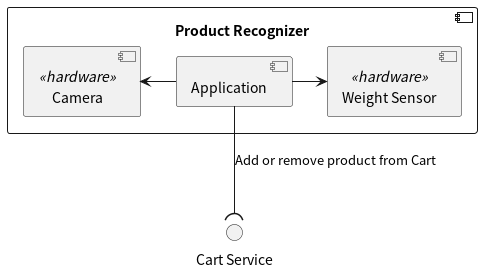
\includegraphics[width=0.7\textwidth]{./images/diagrams/ProductRecognizer.png}
	\caption[]{}
	\fonte{Own work}
	\label{fig:dummy}
\end{figure}

Each of these sub-components will be described in more detail in the next subsections.

\subsection{Weight Sensor}

For the Weight Sensor, we've used two main hardware components, shown on Figure \ref{fig:weighttesting}:
\begin{itemize}
    \item  A 10 Kilogram Load Cell
    \item HX711 Integrated Circuit
\end{itemize}

The HX711 is a 24-bit analog-to-digital converter (\sigla{ADC}{Analog-to-Digital Converter})
capable of outputting data in a serial interface \cite{Avia2022}.

It has two channels for analog input with channel A having programmable gains of 128 or 64 and
can function using both 3.3V and 5V standard digital voltage levels.

One of its advantages is is that there's no need to program internal registers,
all controls to the chip are through its pins. Additionally, it consumes only
1,5 mA under normal operation and has an on-chip power supply for the connected
load cell, making it a great choice for our prototype.

\begin{figure}[H]
	\centering
	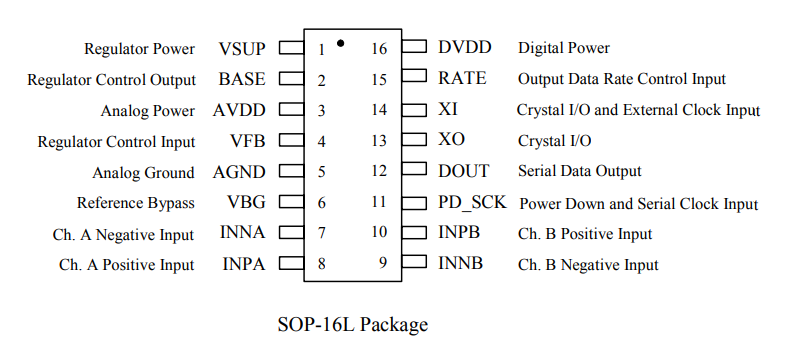
\includegraphics[width=0.9\textwidth]{./images/hx711-pinout.png}
	\caption[HX711 Pinout for the SOP-16L package]{HX711 Pinout for the SOP-16L package}
    \fonte{\cite{Avia2022}}
	\label{fig:architecture}
\end{figure}

\begin{figure}[H]
	\centering
	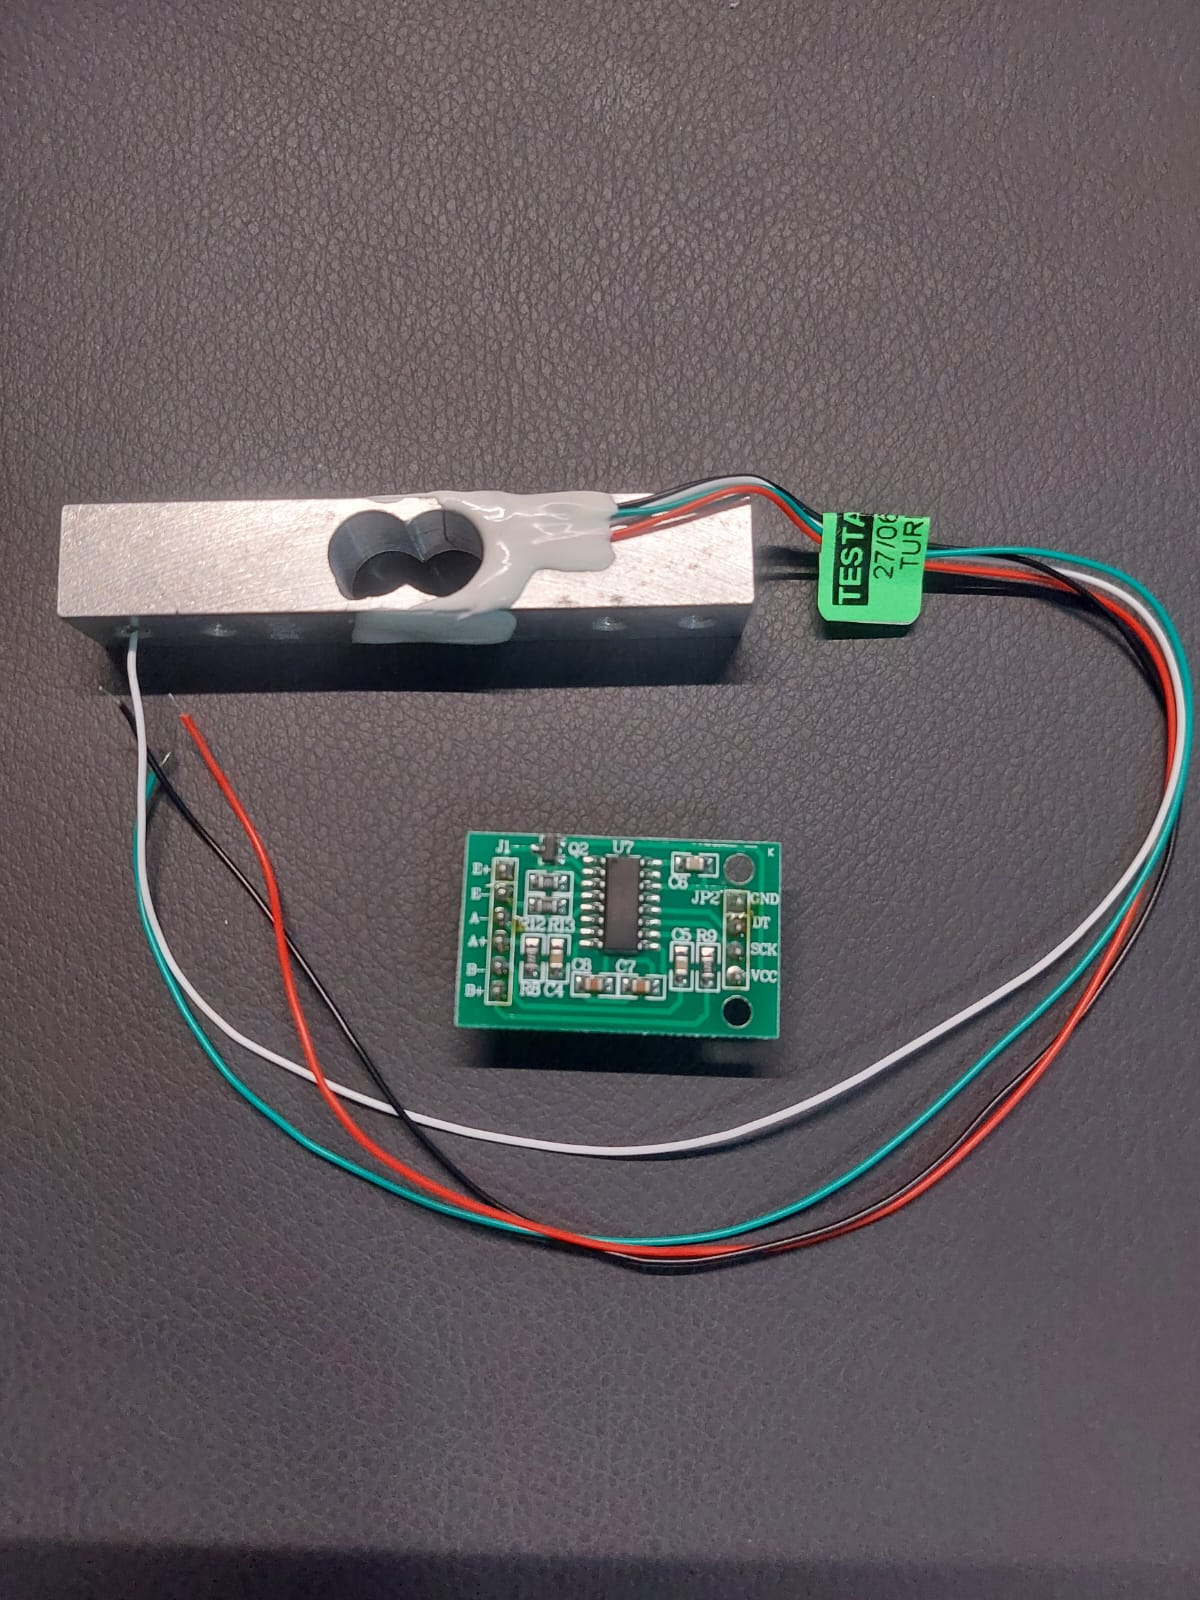
\includegraphics[width=0.4\textwidth]{./images/hx711.jpeg}
	\caption[HX711 breakout board and load cell]{HX711 breakout board and load cell}
	\fonte{Own work}
	\label{fig:weighttesting}
\end{figure}

The HX711 integrated circuited comes in a breakout board that contains the necessary passive components
and includes the pin headers for connecting with other boards.

\begin{figure}[H]
	\centering
	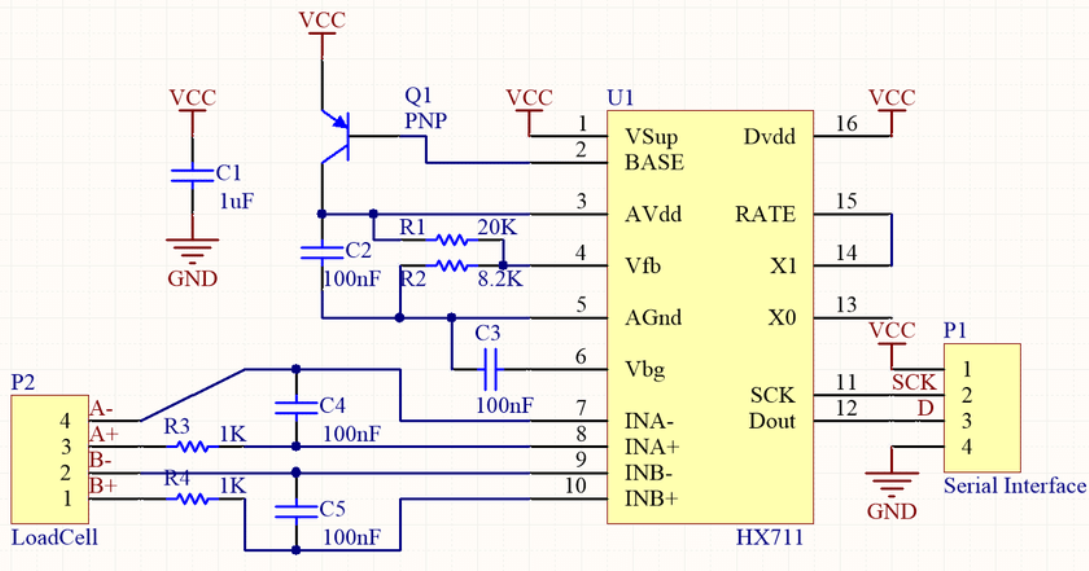
\includegraphics[width=0.8\textwidth]{./images/hx711circuit.png}
	\caption[Typical HX711 circuit]{Typical HX711 circuit}
    \fonte{\cite{Ross2019}}
\end{figure}

The Raspberry Pi board was connected to the HX711 through its GPIO pins,
allowing it to obtain the sensor readings through the serial interface. The
protocol used does not follow any known standard and can be
described as a \textit{Non-I2C compliant two-wire
protocol}\footnote{https://github.com/queuetue/Q2-HX711-Arduino-Library}.

An open-source driver implementation was used\footnote{https://github.com/tatobari/hx711py}, 
which included all the necessary features for the prototype.

As shown on Figure \ref{fig:weighttesting}, the load cell requires a minimal
mechanical assembly to be tested properly, and for that two small wood plates
were used to secure the load cell and breakout board during development.

\begin{figure}[H]
	\centering
	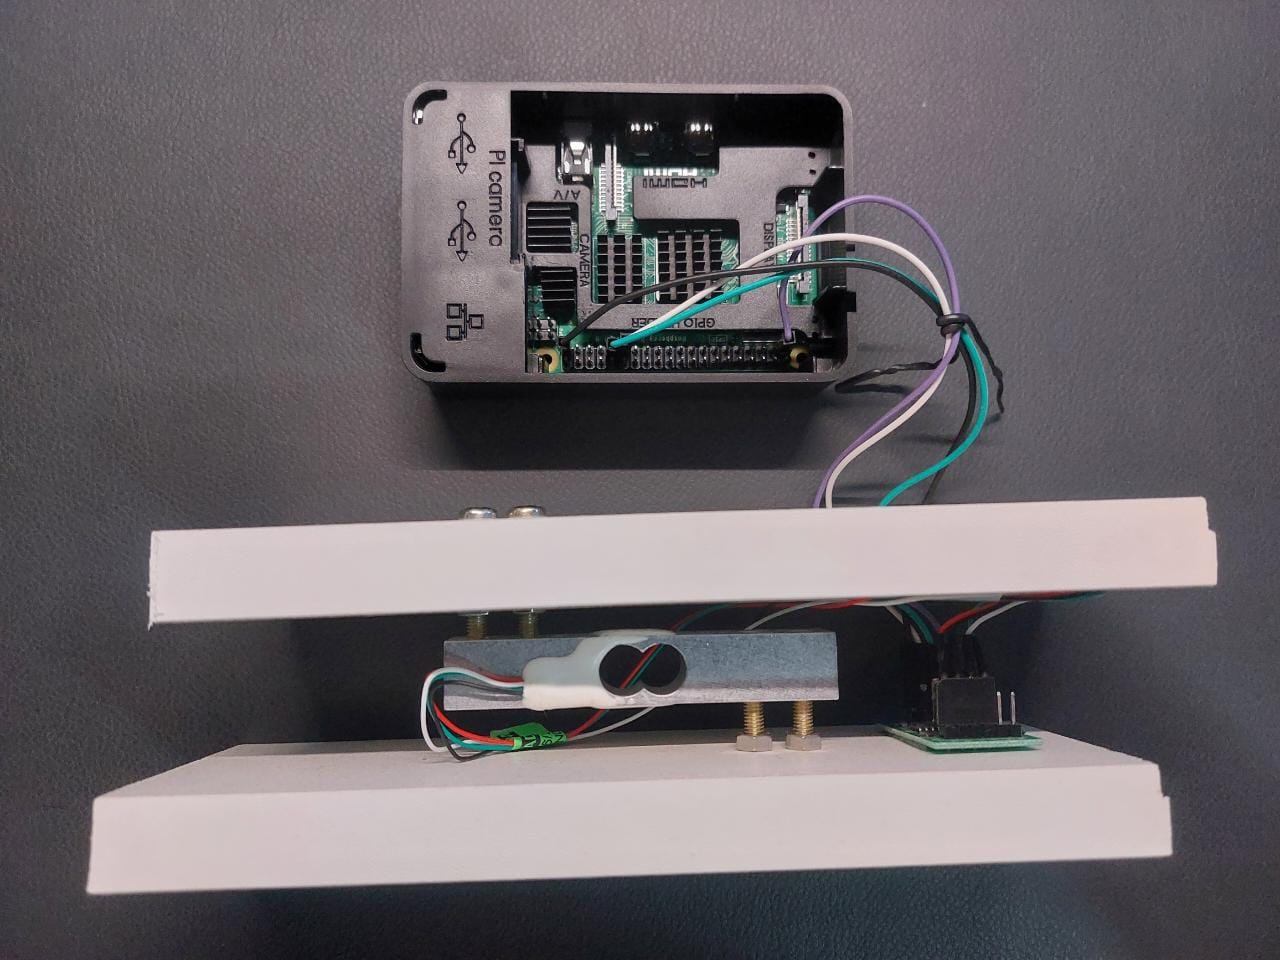
\includegraphics[width=0.7\textwidth]{./images/raspberrypiwithloadcell.jpeg}
    \caption[Assembly used during development, including the Raspberry Pi, HX711 and load cell assembly]{Assembly used during development, including the Raspberry Pi, HX711 and load cell assembly}
	\fonte{Own work}
	\label{fig:dummy}
\end{figure}

\subsection{Camera}

In order to obtain a video feed to run object detection on, a camera system was
required. For that, a standard consumer webcam was used for its reduced cost
and good operating system driver support.

The webcam used was a Microsoft LifeCam
Cinema\footnote{https://www.microsoft.com/pt-BR/accessories/products/webcams/lifecam-cinema},
capable of capturing video in 720p up to 30\sigla{FPS}{Frames Per Second}, more
than enough for our prototyping requirements.

\begin{figure}[H]
	\centering
	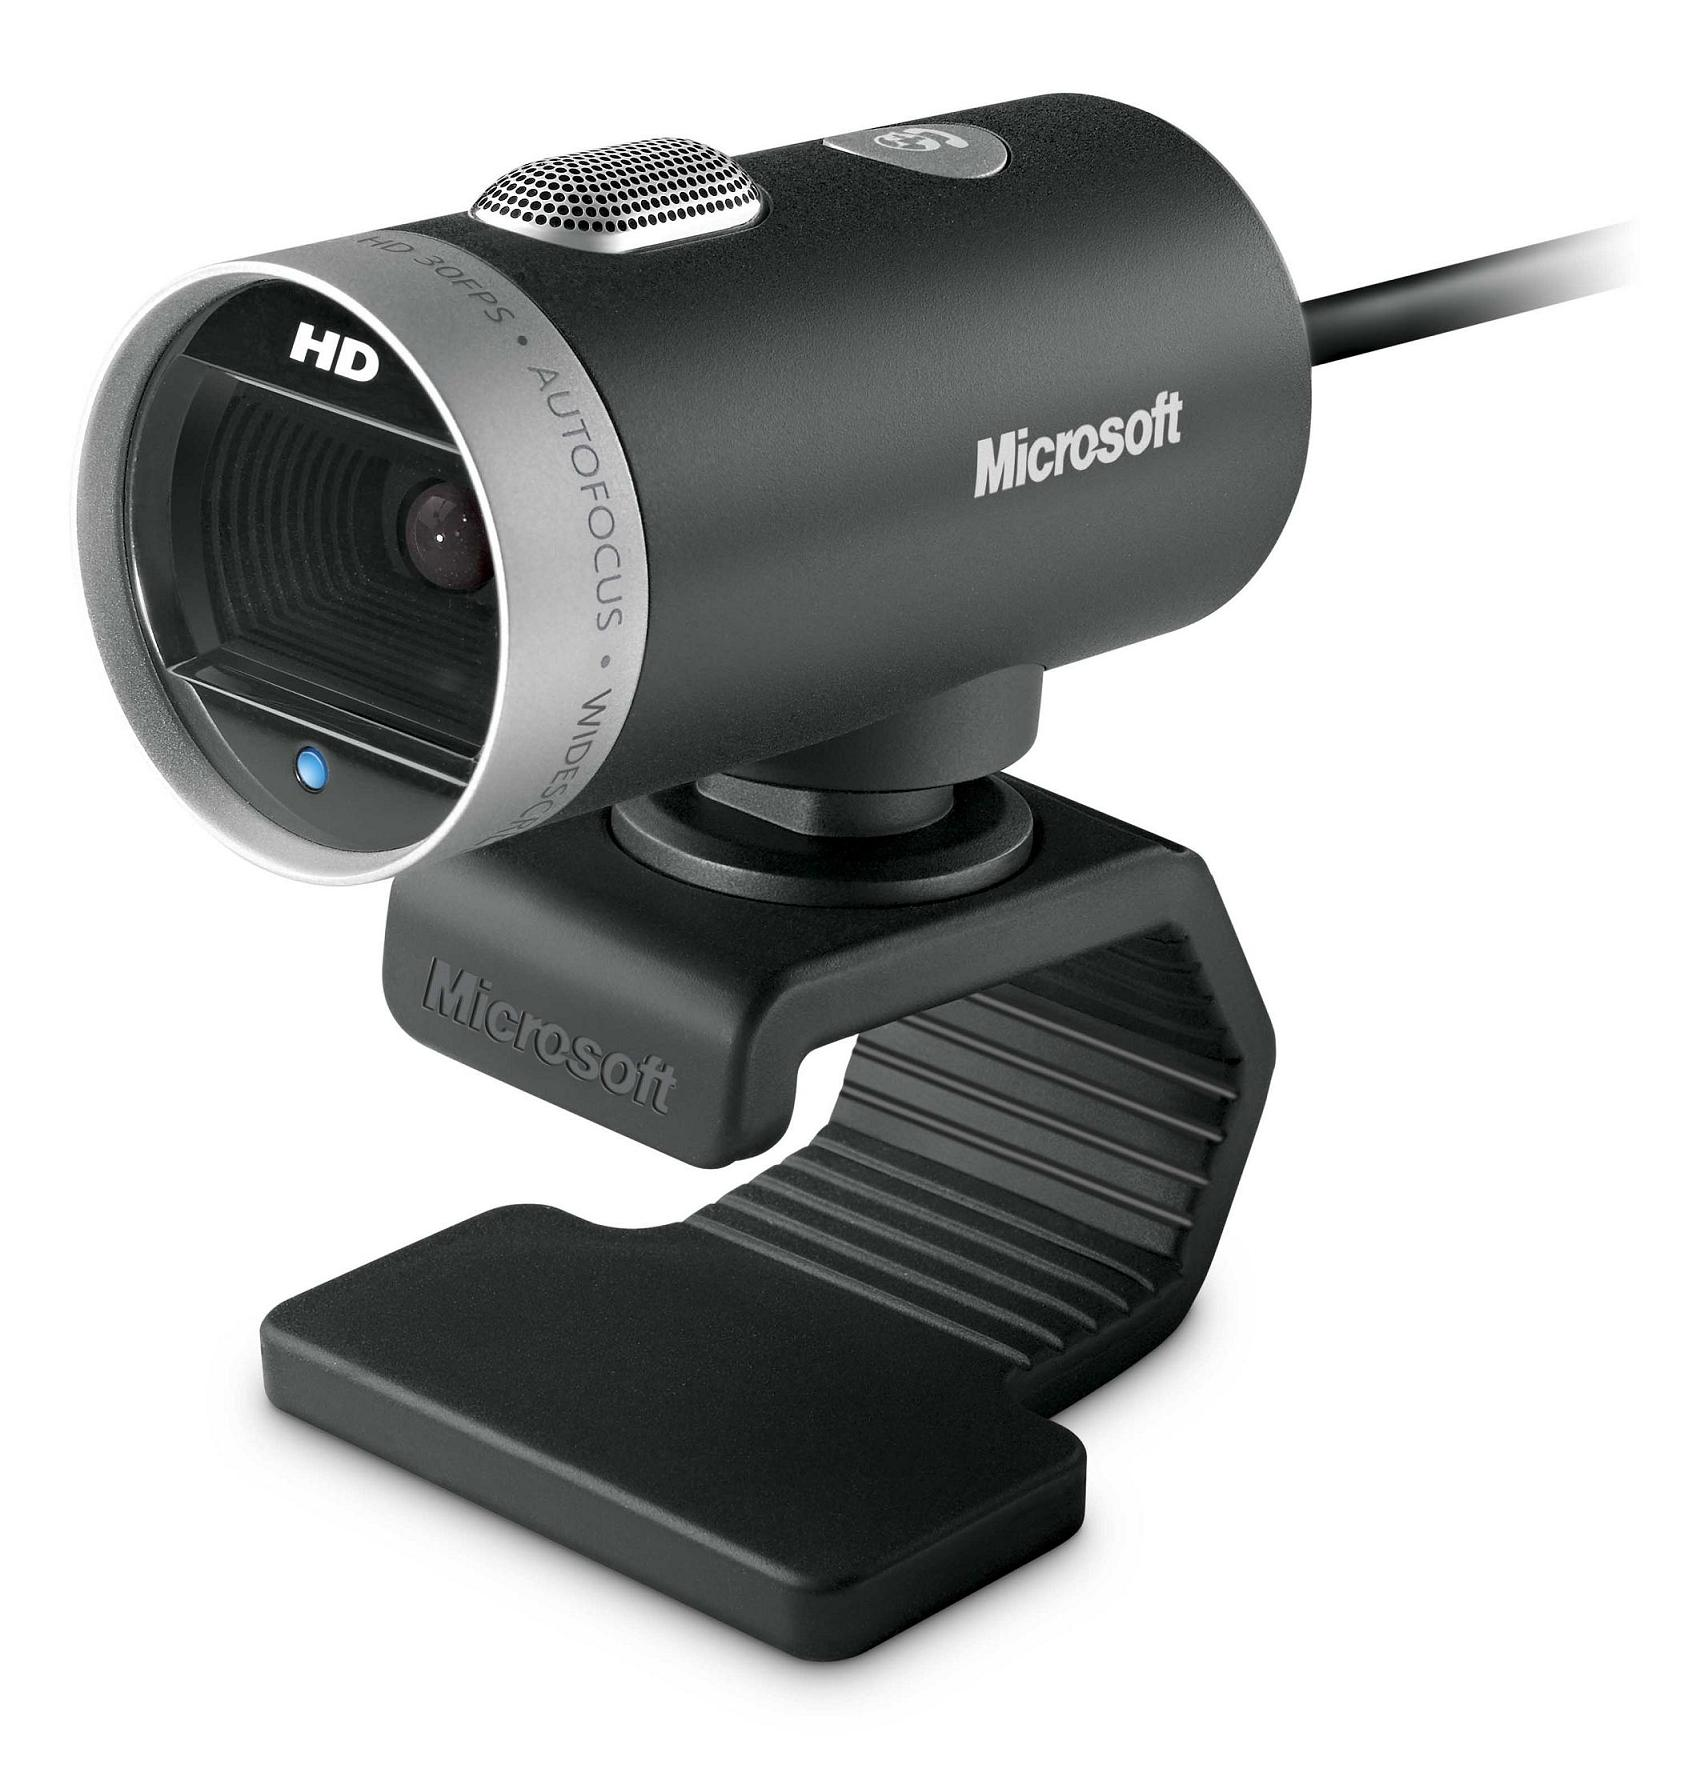
\includegraphics[width=0.3\textwidth]{./images/webcam.jpg}
    \caption[Microsoft LifeCam Cinema Webcam used]{Microsoft LifeCam Cinema Webcam used}
	\fonte{Microsoft}
\end{figure}

\subsection{Application}

Developed in the Python\footnote{https://python.org} programming language, the
Product Recognizer application will provide the compute capabilities to apply
our business logic for processing the video feed provided by the camera and the
readings from the weight sensor.

The Python language was chosen for its vast tooling for working with computer
vision, sensors and interacting with the Raspberry Pi's built-in devices. The
language has also became a \textit{lingua franca} in the Machine Learning and
Data Science community as shown by volume of publications using it in the last
decade \cite{Wes2017,Joel2019,Andreas2016}.

The Product Recognizer application also uses a multi-threaded design to allow
concurrent processing, an important factor when considering the amount
\sigla{I/O}{Input/Output} operations performed.

Since Python's threading implementation does not allow for multiple threads to
execute in parallel -- i.e. at the same time -- a multi-process design could take
better advantage of the four available processing cores in the Raspberry Pi CPU
but that path was not explored and will be left for future iterations.

The three threads created are described below:
\begin{itemize}
    \item Frame Reader Thread: Responsible for reading frames from the Camera and making them available to the Main Thread.
    \item Main Thread: Responsible for bootstraping the application - including creating the other threads - and executing the main loop of
        object detection.
    \item Product Recognizer Thread: Responsible for applying the business logic using the objects detected and the weight sensor readings.
\end{itemize}

These threads communicate in synchronous and asynchronous means to achieve the overall goal of processing video and sensor data, as shown on Figure \ref{fig:threads}.

\begin{figure}[H]
	\centering
	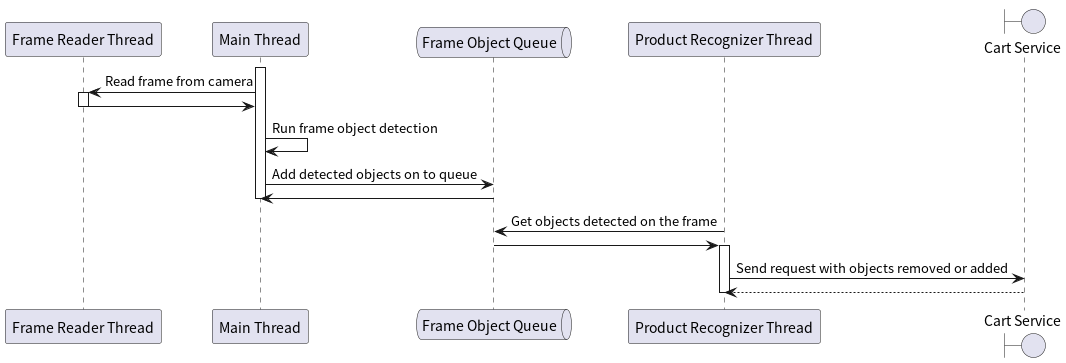
\includegraphics[width=1\textwidth]{./images/Product Recognizer Thread communication.png}
	\caption[Thread communication for the Product Recognizer Appplication]{Thread communication for the Product Recognizer Application}
	\fonte{Own work}
	\label{fig:threads}
\end{figure}

\begin{lstlisting}[language=Python,caption={Loop of the Main Thread. Some details were ommitted for the sake of brevity},label={lst:main}]
while True:
  try:
    # Get frame from camera, provided by Frame Reader thread
    frame = stream.read_frame()

    # Preprocess and run object detection
    input = preprocessor.process(frame)
    detector.infer(input)

    # Filter objects by their class and confidence threshold
    objects = detector.get_objects()
    filtered_objects = object_filter.filter(objects)

    # Add filtered objects to the queue
    frame_objects_queue.put(filtered_objects)
\end{lstlisting}

As shown on Listing \ref{lst:main} and on Figure \ref{fig:threads}, the Main
thread will do the computational work to fetch the frames from the camera that
were read by the Frame Reader thread, pre-process and run the object detection
model in it. The objects are then filtered and then added to a message queue
that will be used by the Product Recognizer thread to apply our business logic.

\subsection{Product Recognizer Thread}

The Product Recognizer Thread is responsible for applying the main business
logic of detecting the addition and removal of products by leveraging the
objects detected in the frame and the readings provided by the weight sensor.

The thread will execute an infinite loop to constantly observe the objects
detected in the frame and the weight readings to detect product additions
and removals.

It uses two main variables to keep track of the current state:
\begin{itemize}
    \item A dictionary of which products are present in the cart and their count.
    \item The weight associated with the products present in the cart.
\end{itemize}

The first important step in the thread's logic is the \textit{Frame Diff}. This step 
calculates the difference in terms of the objects detected in the current 
and previous frames (e.g. whether objects were added, removed, or remain the same) 
and store it in a dictionary data structure\footnote{https://docs.python.org/3/tutorial/datastructures.html\#dictionaries},
by comparing the stored product dictionary and the received list of frame
objects from the Main Thread.

\begin{figure}[H]
	\centering
	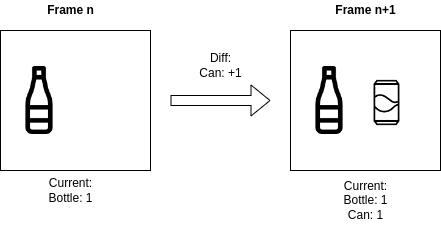
\includegraphics[width=0.8\textwidth]{./images/diagrams/framediff.png}
	\caption[Illustration of the frame diff'ing scheme]{Illustration of the frame diff'ing scheme. A can was added on frame $n+1$ and therefore will generate a diff of one can. If the reading from the weight sensor matches the expected one, the product will be added to the cart.}
	\fonte{Own work}
    \label{fig:diff}
\end{figure}

Given the frame object diff, it is then possible to calculate an expected
weight change based on the weight of each item - and their quantity - contained
in the diff. The expected weight difference is then compared to the actual
one obtained from the weight sensor, considering a configurable tolerance.

In this scenario, the weight readings are used as a filter and act as a
\textit{commit} step for differences detected in the frame objects. This way, objects are not
added or removed from the cart simply by appearing or disappearing from the frame.

In the example show in Figure \ref{fig:diff}, if the illustrated can weights an expected 400 grams, the weight
difference expected should be close to 400 grams. If the weight difference does not match the expected
one, the object will not be considered for addition or removal. 

A more detailed activity diagram of the logic executed in the Product Recognizer thread loop is
shown in Figure \ref{fig:activity}.

\begin{figure}[H]
	\centering
	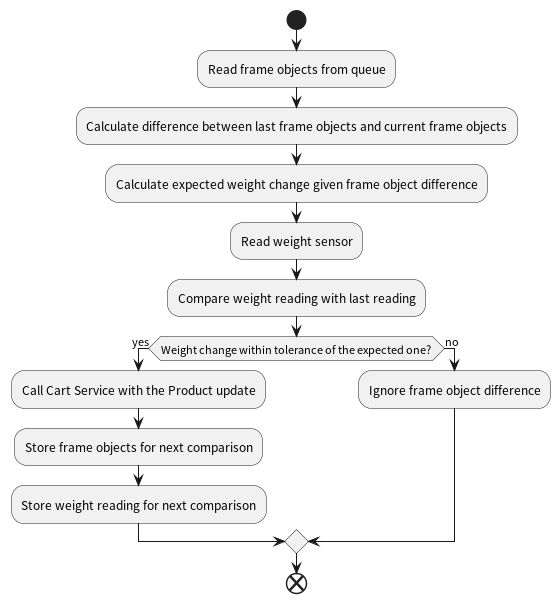
\includegraphics[width=0.8\textwidth]{./images/Product Recognizer Activity.png}
	\caption[Activity diagram for the Product Recognizer thread]{Activity diagram for the Product Recognizer thread}
	\fonte{Own work}
    \label{fig:activity}
\end{figure}

\begin{lstlisting}[language=Python,caption={Product Recognizer thread logic}]
objects = self.queue.get_nowait()

# Preprocessing step just to format data
current_frame_objects = self.__build_object_dict(objects)

# Calculate the frame diff using the last and current frame objects
frame_diff = self.__get_frame_diff(
    current_frame_objects, self.last_frame_objects
)

if len(frame_diff) == 0:
    self.log.info("empty diff")
    continue

# Get current weight reading
weight_reading = self.weight_sensor.get_reading(samples=5)

for label, count in frame_diff.items():
    if not self.__valid_weight_difference(label, count, weight_reading):
        self.log.info("ignoring, not valid weight difference")
        continue

    # Send request to cart service
    self.__call_cart_service(label, count)

    # Update stored state
    self.last_weight_reading = weight_reading
    self.last_frame_objects[label] = current_frame_objects[label]
    if self.last_frame_objects[label] == 0:
        del self.last_frame_objects[label]
\end{lstlisting}

\subsection{Object Detection Model}

To actually execute the Product Recognizer logic, a object detection model was
in order and for that the first step was to actually collect the training data.

It was collected and labelled using Edge
Impulse\footnote{https://www.edgeimpulse.com/}, a development platform for
Machine Learning on Edge devices. A total of 1000 photos were taken using the
Data Collection feature of the Edge Impulse Studio, using the same webcam that
is used for the inference in our final product.

\begin{figure}[H]
	\centering
	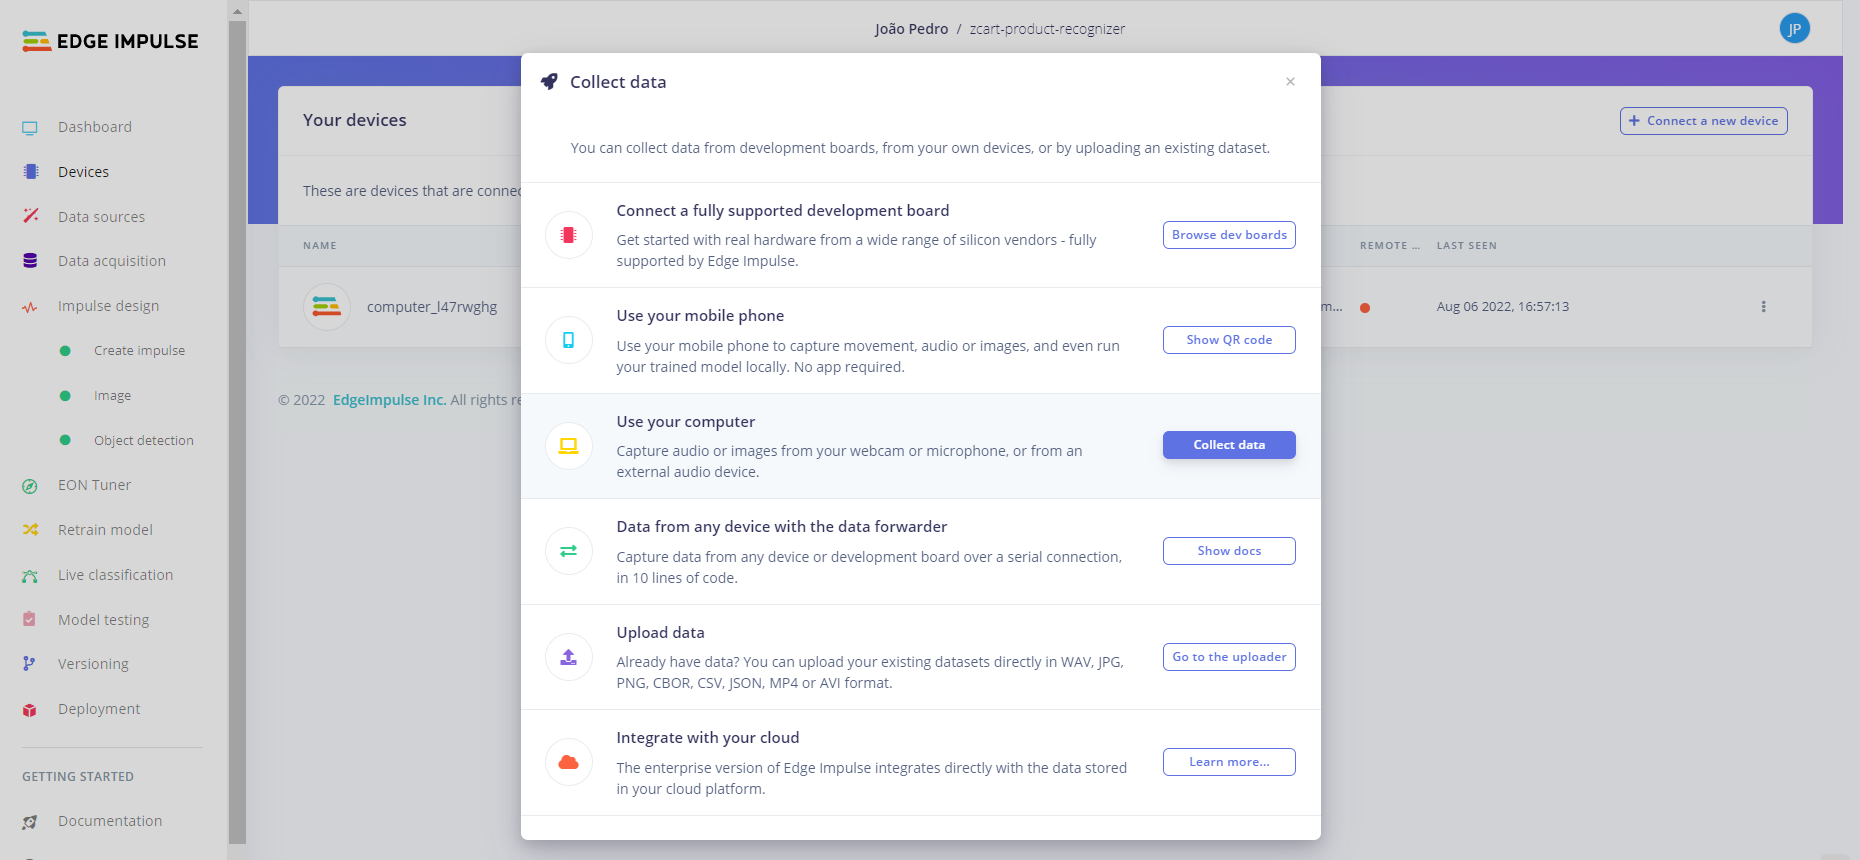
\includegraphics[width=0.75\textwidth]{./images/edge-impulse-collect-data.png}
	\caption[Collecting Data in Edge Impulse]{Collecting Data in Edge Impulse}
	\fonte{Edge Impulse}
    \label{fig:diff}
\end{figure}

The pictures were then were labelled using the Labelling Queue\footnote{https://docs.edgeimpulse.com/docs/edge-impulse-studio/data-acquisition/labeling-queue}
feature of Edge Impulse, which allowed us to draw Bounding Boxes around the desired objects for detection.

\begin{figure}[H]
	\centering
	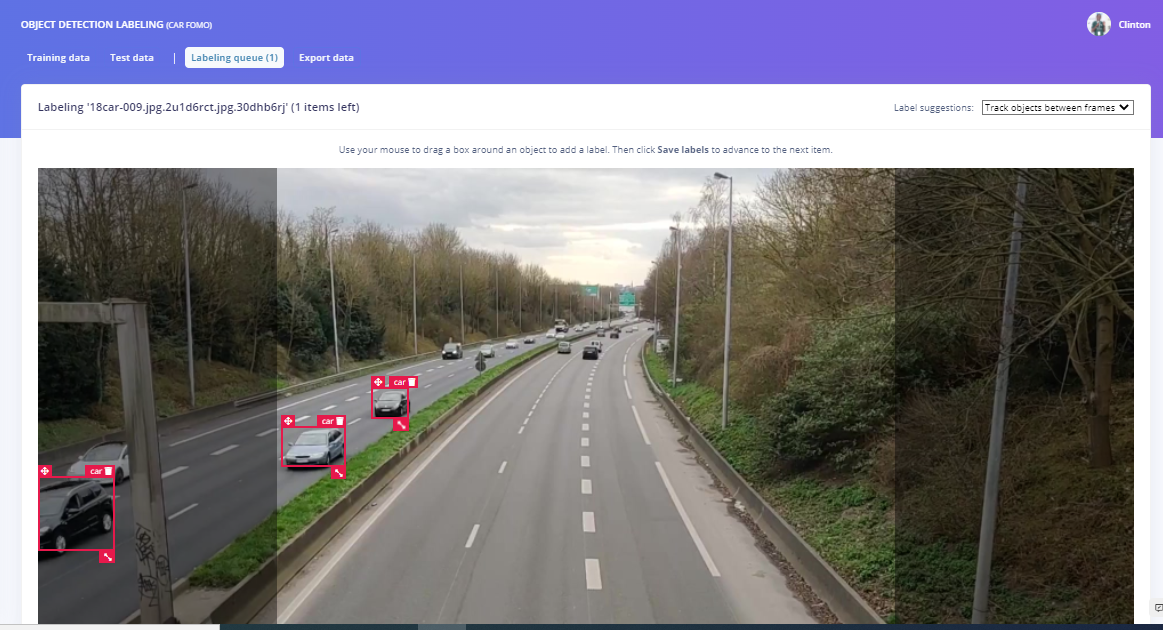
\includegraphics[width=0.75\textwidth]{./images/edge-impulse-labelling-queue.png}
	\caption[Labelling Queue in Edge Impulse]{Labelling Queue in Edge Impulse}
	\fonte{Edge Impulse}
    \label{fig:diff}
\end{figure}

The raw pictures and bounding boxes were then exported from Edge Impulse such
that we could pre-process the data and model our custom object detection
algorithm using the Python programming language. The pictures were exported in
their raw JPEG\footnote{Defined in ISO/IEC 10918}  file format, comprised in a
ZIP folder. The bounding boxes were exported in the format of a JSON file
containing the coordinates for the boundaries and the metrics for each picture,
allowing us to easily reconstruct the bounding boxes for each object in each
image using programming instructions. The files were then loaded to a Cloud
Object Storage Bucket in AWS \footnote{https://aws.amazon.com/}, making it
easier for us to access the data by importing it from the web using any
programming language.

\begin{lstlisting}[caption={Bounding boxes coordinates file exported from Edge Impulse},label={lst:boundingBoxCoordinates}]
	{
		"version": 1,
		"type": "bounding-box-labels",
		"boundingBoxes": {
		  "im1.jpg": [
			{
			  "label": "blue_pens",
			  "x": 120,
			  "y": 265,
			  "width": 172,
			  "height": 207
			},
			{
			  "label": "card_deck",
			  "x": 285,
			  "y": 120,
			  "width": 136,
			  "height": 247
			}
		  ],
		  "im2.jpg": [
			(...)
		  ]
		}
	}
\end{lstlisting}

The development environment used for writing the code for training our custom model
was Google Colab\footnote{https://colab.research.google.com/}, and the programming language 
of choice was Python. 
Google Colab consists on a web-based interface that allows developers
to use Google's infrastructure (with GPUs and TPUs) for writing and executing code.

\begin{figure}[H]
	\centering
	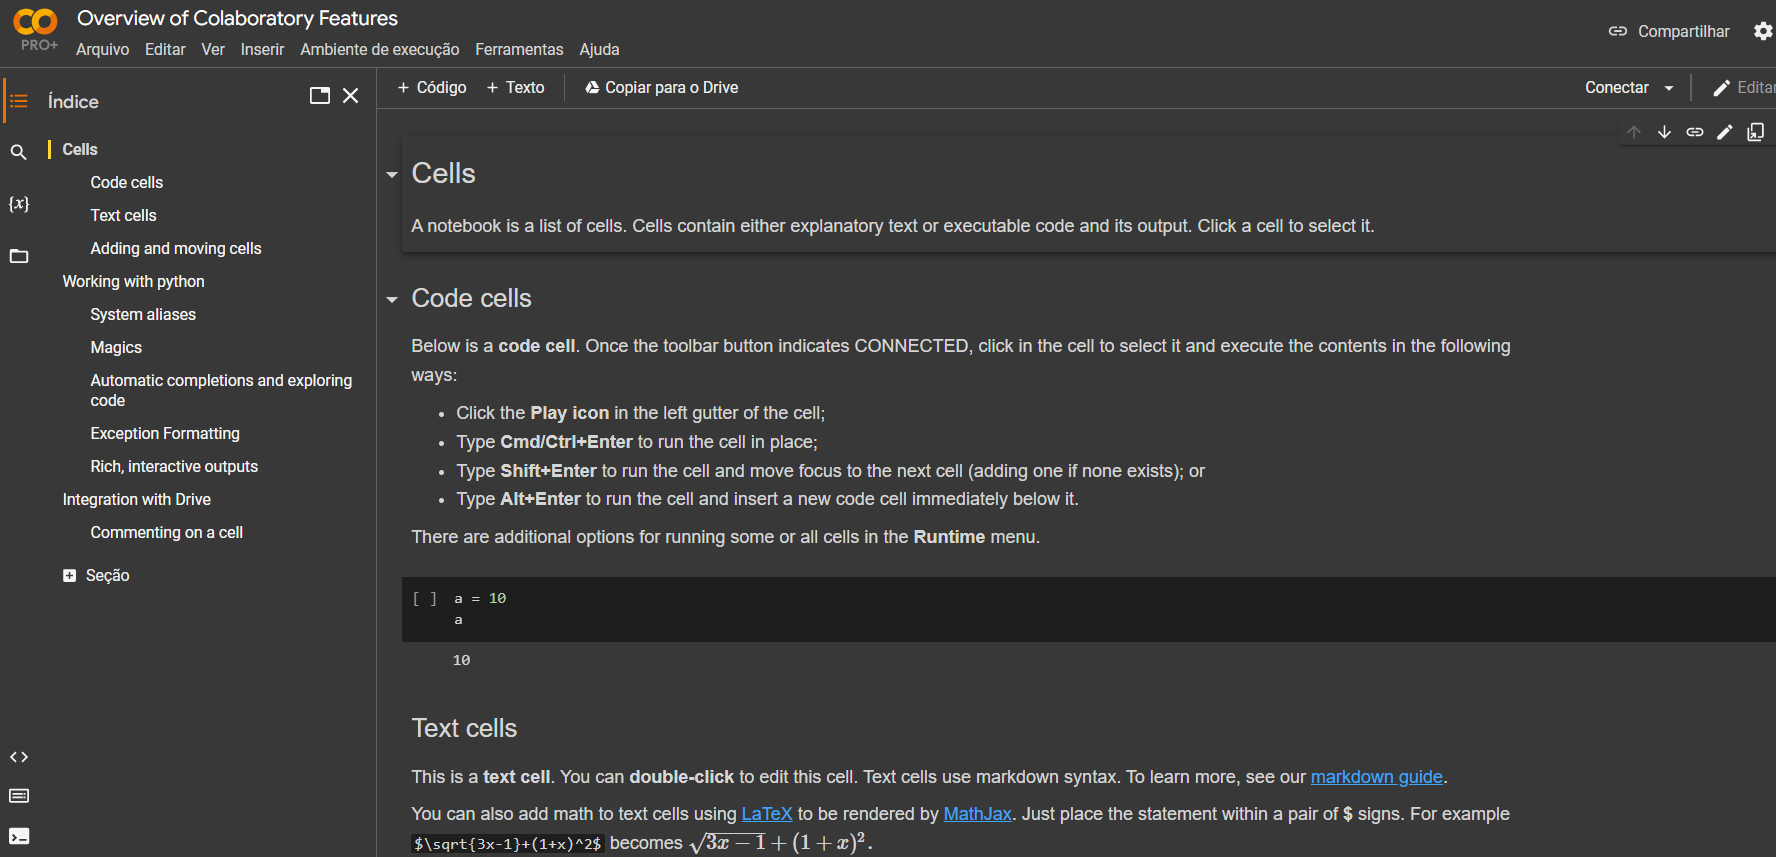
\includegraphics[width=0.7\textwidth]{./images/google-colab.png}
	\caption[Google Colab - Overview of Colaboratory Features]{Google Colab - Overview of Colaboratory Features}
	\fonte{Google\footnote{https://colab.research.google.com/notebooks/basic\_features\_overview.ipynb}}
    \label{fig:diff}
\end{figure}

The Edge Impulse files were loaded from our cloud object storage bucket, and then manipulated in Python
from Google Collab such that we could utilize the images and bounding box coordinates for training
our model.

We decided to use Google's TensorFlow\footnote{https://www.tensorflow.org/} framework to train our 
models, as it is one of the most popular frameworks employed in the Industry for training AI models
and also because it features a lightweight library called TensorFlow Lite\footnote{https://www.tensorflow.org/lite}, 
which is appropriate for creating efficient edge and mobile AI models considering the 
typical hardware constraints from these types of devices.

To train our model, we used the TensorFlow Lite's ModelMaker API\footnote{https://www.tensorflow.org/lite/models/modify/model\_maker} 
for Object Detection, which simplifies the process of training our models by breaking down the most
complex concepts of deep learning into parameterized objects and methods, allowing us to spend
more time on the pre-processing steps and on experimenting with different network configurations
to improve the model's accuracy. 

As of writing this work, the ModelMaker API only has compatibility
with the EfficientDet family of architectures \cite{Mingxing2020} for training
Deep Learning models for Object Detection. The EfficientDet family is efficient
for object recognition in edge devices, altough contemporany architectures,
such as the YOLOv5 and its successors, can have better performance.

\begin{figure}[H]
	\centering
	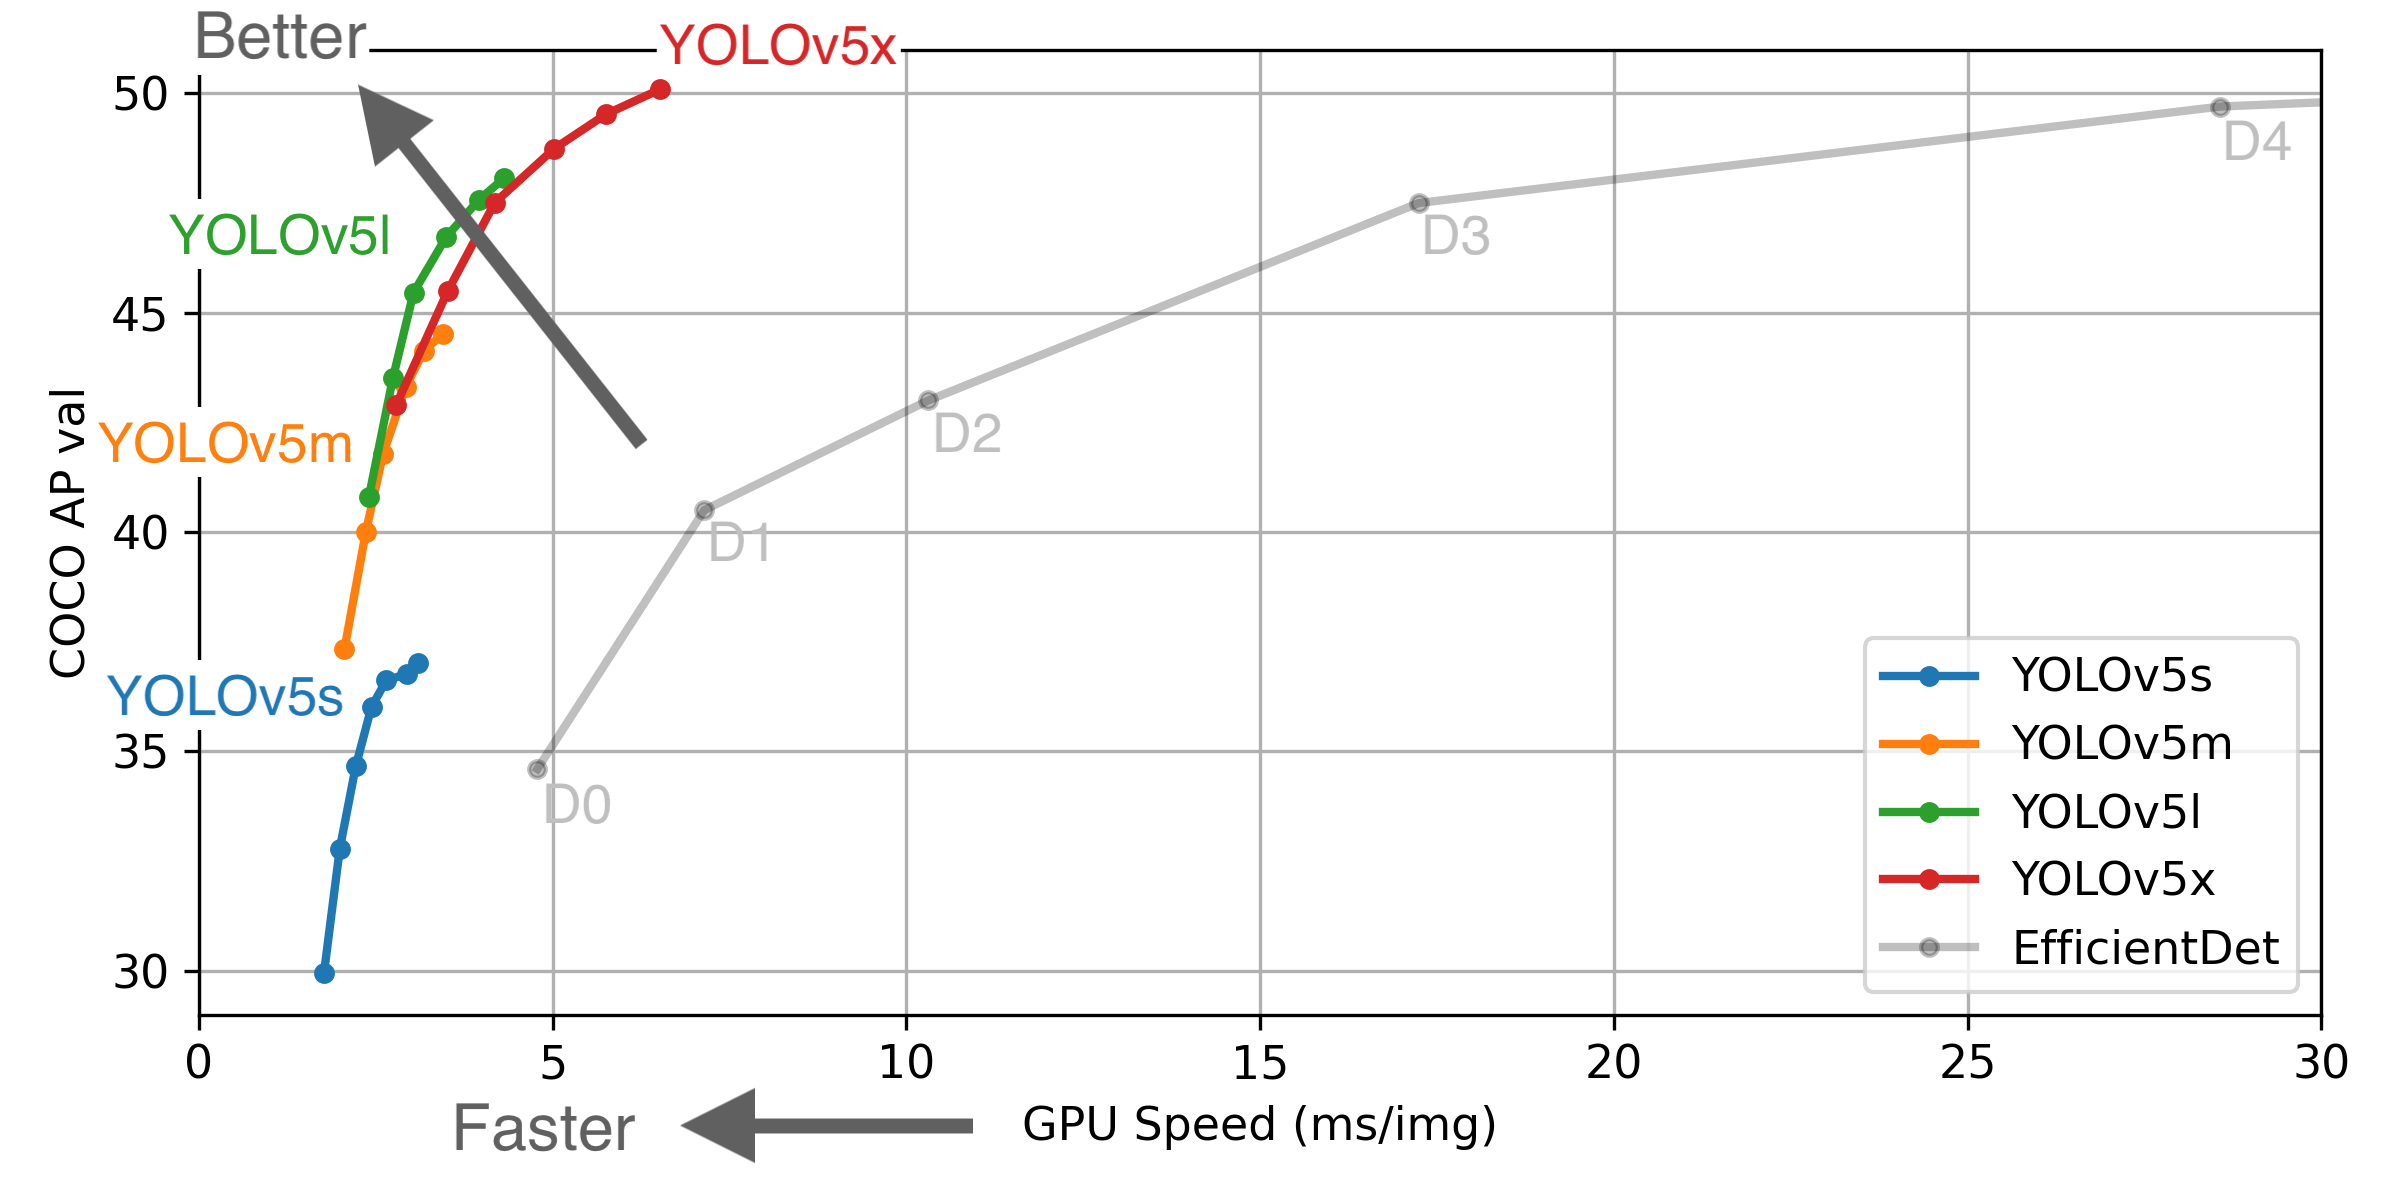
\includegraphics[width=0.6\textwidth]{./images/yolo-efficientdet-comparison.png}
	\caption[YOLOv5 vs EfficientDet - Performance Comparison]{YOLOv5 vs EfficientDet - Performance Comparison}
	\fonte{YOLOv5 Release Notes\footnote{https://github.com/ultralytics/yolov5/releases/tag/v4.0}}
    \label{fig:diff}
\end{figure}

Our initial plan was to use the YOLOv5 architecture, but since its
implementation is not native to TensorFlow Lite, it would require us to create
additional wrappers around the outputs of the YOLOv5 network to get it working
as expected. Even thought it is possible to convert the models from their
original PyTorch\footnote{https://pytorch.org/} format to a TensorFlow Lite
format, the conversion does not cover some of the features from the original
implementation\footnote{https://github.com/ultralytics/yolov5/issues/1981},
which limits its direct functionality. Similar compatibility issues happen with
the latest YOLO implementations, such as the
YOLOv7\footnote{https://medium.com/geekculture/journey-putting-yolo-v7-model-into-tensorflow-lite-object-detection-api-model-running-on-android-e3f746a02fc4}.
Thus, we have decided to proceed with the TensorFlow Lite's Model Maker API
compatible architectures -- namely the EfficientDet family --  since it would
have taken a considerable time to troubleshoot conversion defects from the YOLO
architecture and all that work wouldn't bring any additional value to our
prototype.

Since our original images were saved in the 640x480 resolution and the expected
input of the EfficientDet network is of 320x320 px, two pre-processing
approaches were tried out for the training dataset: resizing and cropping the
images. The bounding box coordinates and dimensions were also adjusted
accordingly such that the data integrity was preserved. 

\begin{figure}[H]
	\centering
	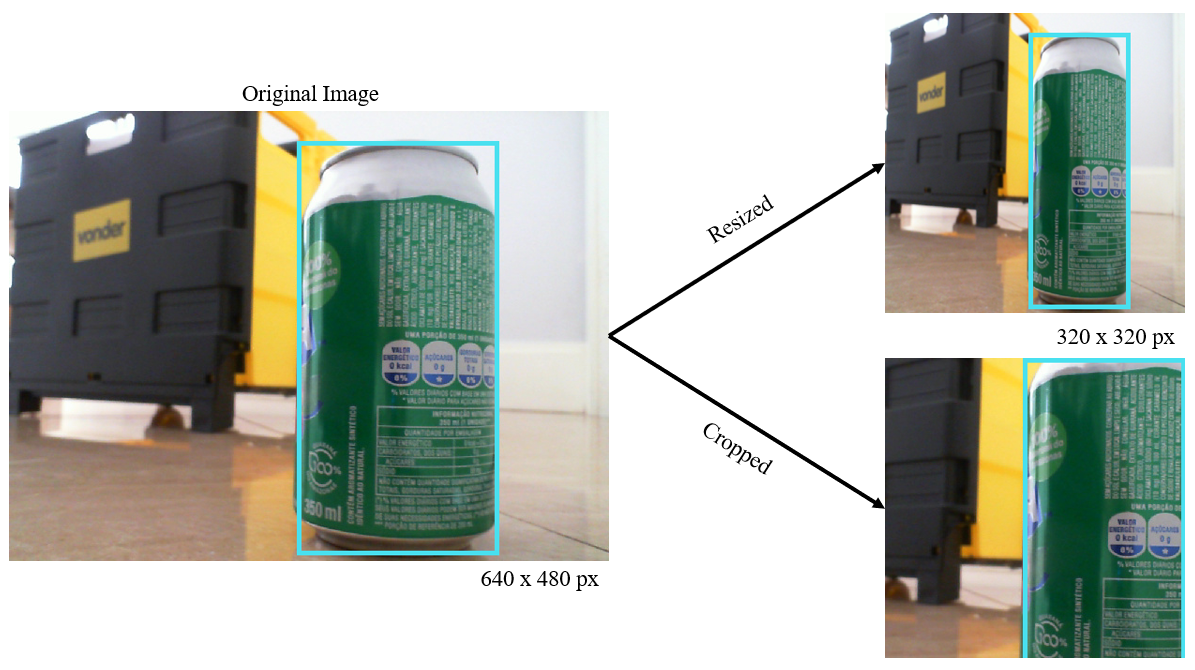
\includegraphics[width=0.7\textwidth]{./images/image_preprocessing.png}
	\caption[Image Preprocessing Strategies]{Image Preprocessing Strategies}
	\fonte{Own work}
\end{figure}

Once the images and bounding boxes were pre-processed, the images were split
into Train, Validation and Test sets; and saved in the standardized format
required by the TensorFlow Lite's Model Maker for Object Detection API for
training, which consists on a Comma Separated Values (\sigla{CSV}{Comma
Separated Values}) in the following structure:

\begin{lstlisting}[caption={CSV format for specifying the Train, Test and Validation 
	image sets for training models using the TensorFlow's Model Maker API for Object 
	Detection},label={lst:csvFormatTrain}]
Template:
set,path,label,x_min,y_min,,,x_max,y_max,,
set,path,label,x_min,y_min,x_max,y_min,x_max,y_max,x_min,y_max

Examples:
TEST,./images_path/im3.png,0.5,0.6,,,0.2,0.9,,
VALIDATION,./images_path/im4.png,label,0.3,0.4,,,0.4,0.8,,
TRAIN,./images_path/im5.png,label,0.3,0.3,0.8,0.8,1.0,0.9,0.1,1.0
TRAIN,./images_path/im6.png,label,0.3,0.1,,,0.3,0.4,,
\end{lstlisting}

Approximately 70\% of the photos shot were moved to the Train set, which is the set used for effectively 
tuning the weights and biases of the custom models; About 21\% were moved to the Validation set, 
being used to understand our model's performance under different training scenarios and steps; 
and the rest was used for testing the custom model after it was trained, which allowed us to 
get unbiased metrics on how it would approximately perform in real life \cite{MluExplain}.

Finally, we defined a programming loop to train different models using the
EfficientDet-D0, EfficientDet-D1, EfficientDet-D2, EfficientDet-D3 and
EfficientDet-D4 architectures; both by applying Transfer Learning on the top of
pre-trained weights from training with the COCO-2017 dataset and by training
the entire networks based in our custom data. 

We ran this entire loop using the cropped images first; and then executed it
using resized images with the EfficientDet-D0, EfficientDet-D1 and
EfficientDet-D2 architectures too, as they were the ones who offered better
performance balance considering our hardware constraints. With that, we came to
have 16 distinct custom models for testing. 

The performance and precision of these models will be discussed in the Results section.

\subsection{Coral Accelerator}

As discussed in Section \ref{sec:TPU}, running DNN inferences on general purpose hardware can be expensive
both in computational and power efficiency terms. 

To alleviate that, we have used the Coral USB Accelerator, a TPU that can be
connected to the Raspberry Pi board through \sigla{USB}{Universal Serial Bus}
and provide significant performance improvements.

\begin{figure}[H]
	\centering
	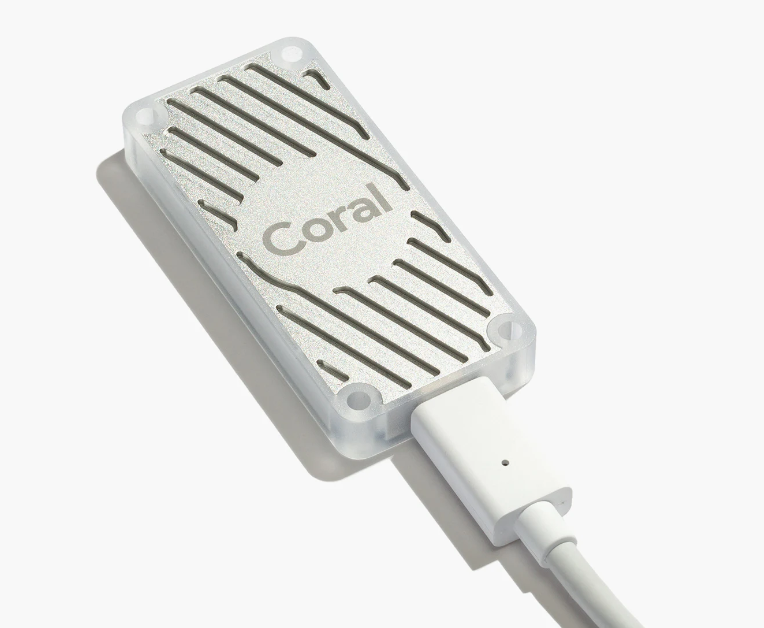
\includegraphics[width=0.4\textwidth]{./images/coralusb.png}
	\caption[Coral USB Accelerator]{Coral USB Accelerator}
	\fonte{Coral.ai}
\end{figure}

To actually utilize the TPU, two important steps needed to be done. The first, is to install
a Linux native library that acts as a driver for the device. The seconds, is that the Tensor Flow Lite 
models need to go through a compilation process\footnote{https://coral.ai/docs/edgetpu/compiler/\#compiler-and-runtime-versions} to actually take advantage of the TPU.

Both of these steps were performed and the results, including performance comparisons 
with and without the TPU are discussed in the Results section.

\section{Mechanical Assembly}

A foldable utility cart was selected as a core
component with two additional wood plates, used for creating a \textit{false
bottom}. Between the plates, the load cell and Raspberry Pi board were secured
in place using bolts, screws and velcro.

\begin{figure}[H]
	\centering
	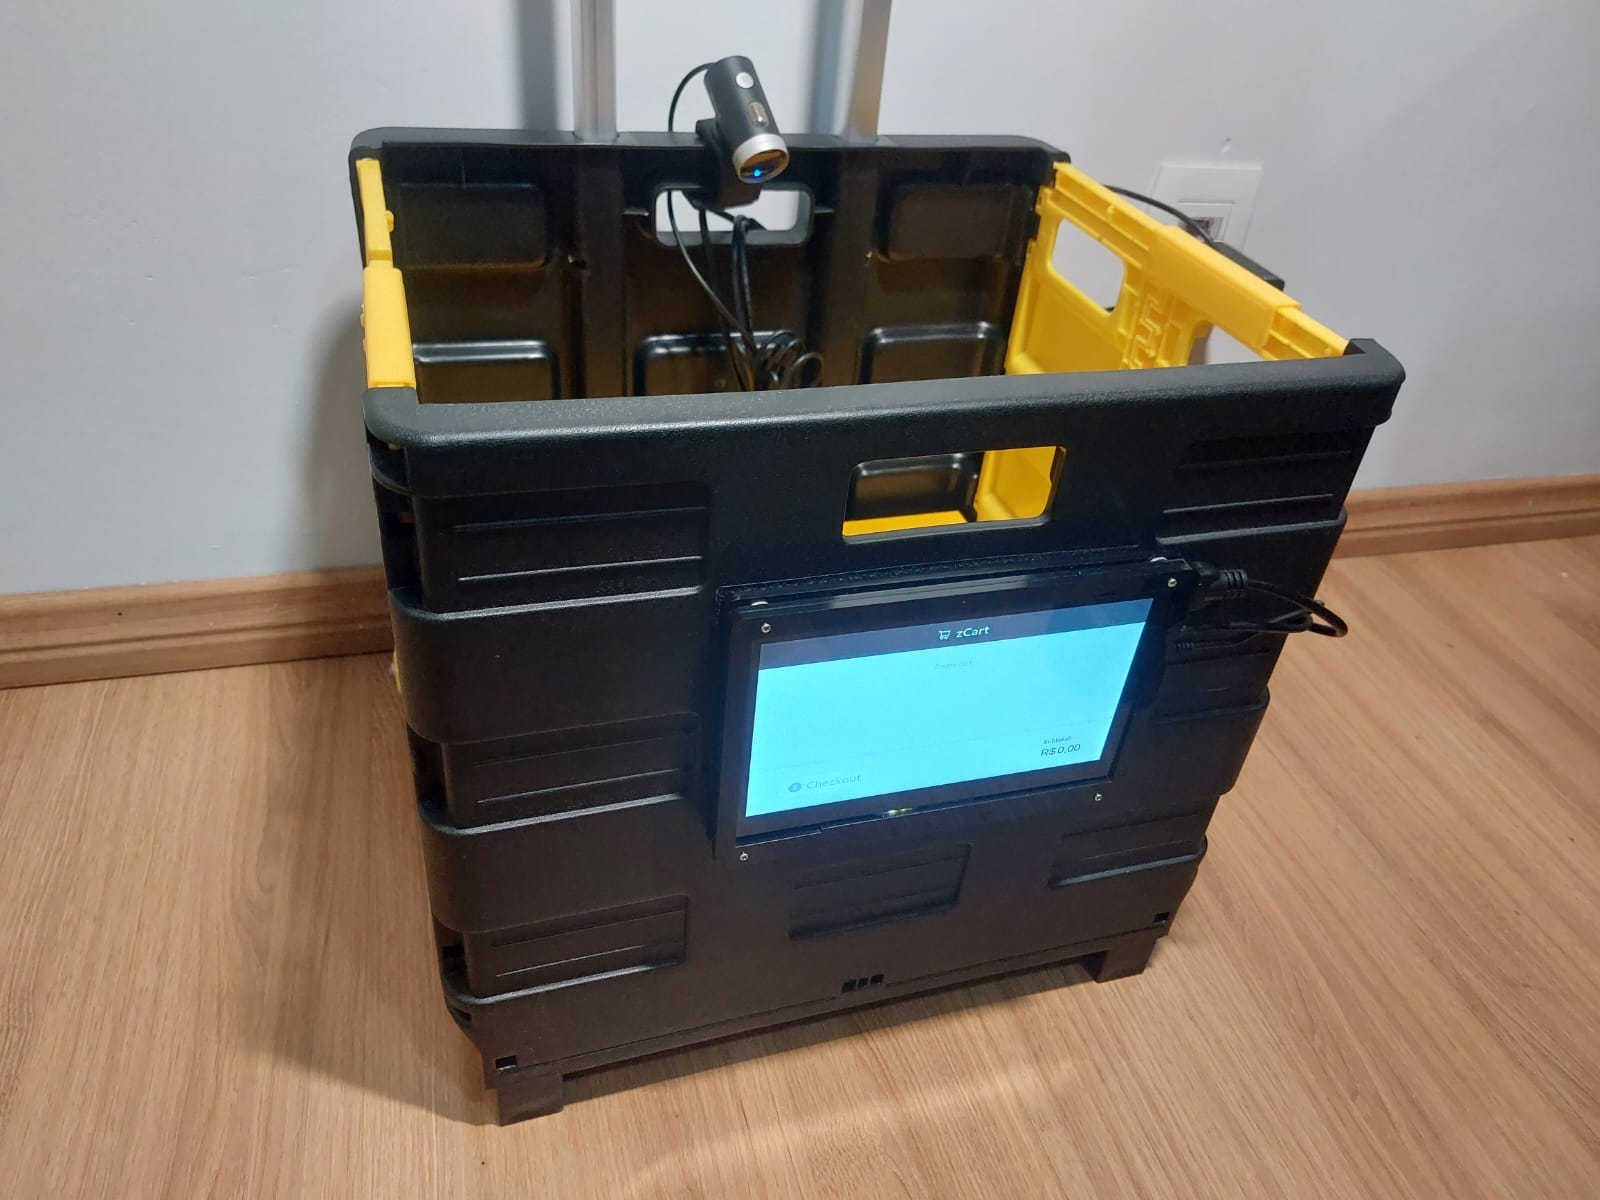
\includegraphics[width=0.75\textwidth]{./images/cart.jpeg}
	\caption[Overall mechanical assembly including the LCD and Camera]{Overall mechanical assembly including the LCD and Camera}
	\fonte{Own work}
\end{figure}

\begin{figure}[H]
	\centering
	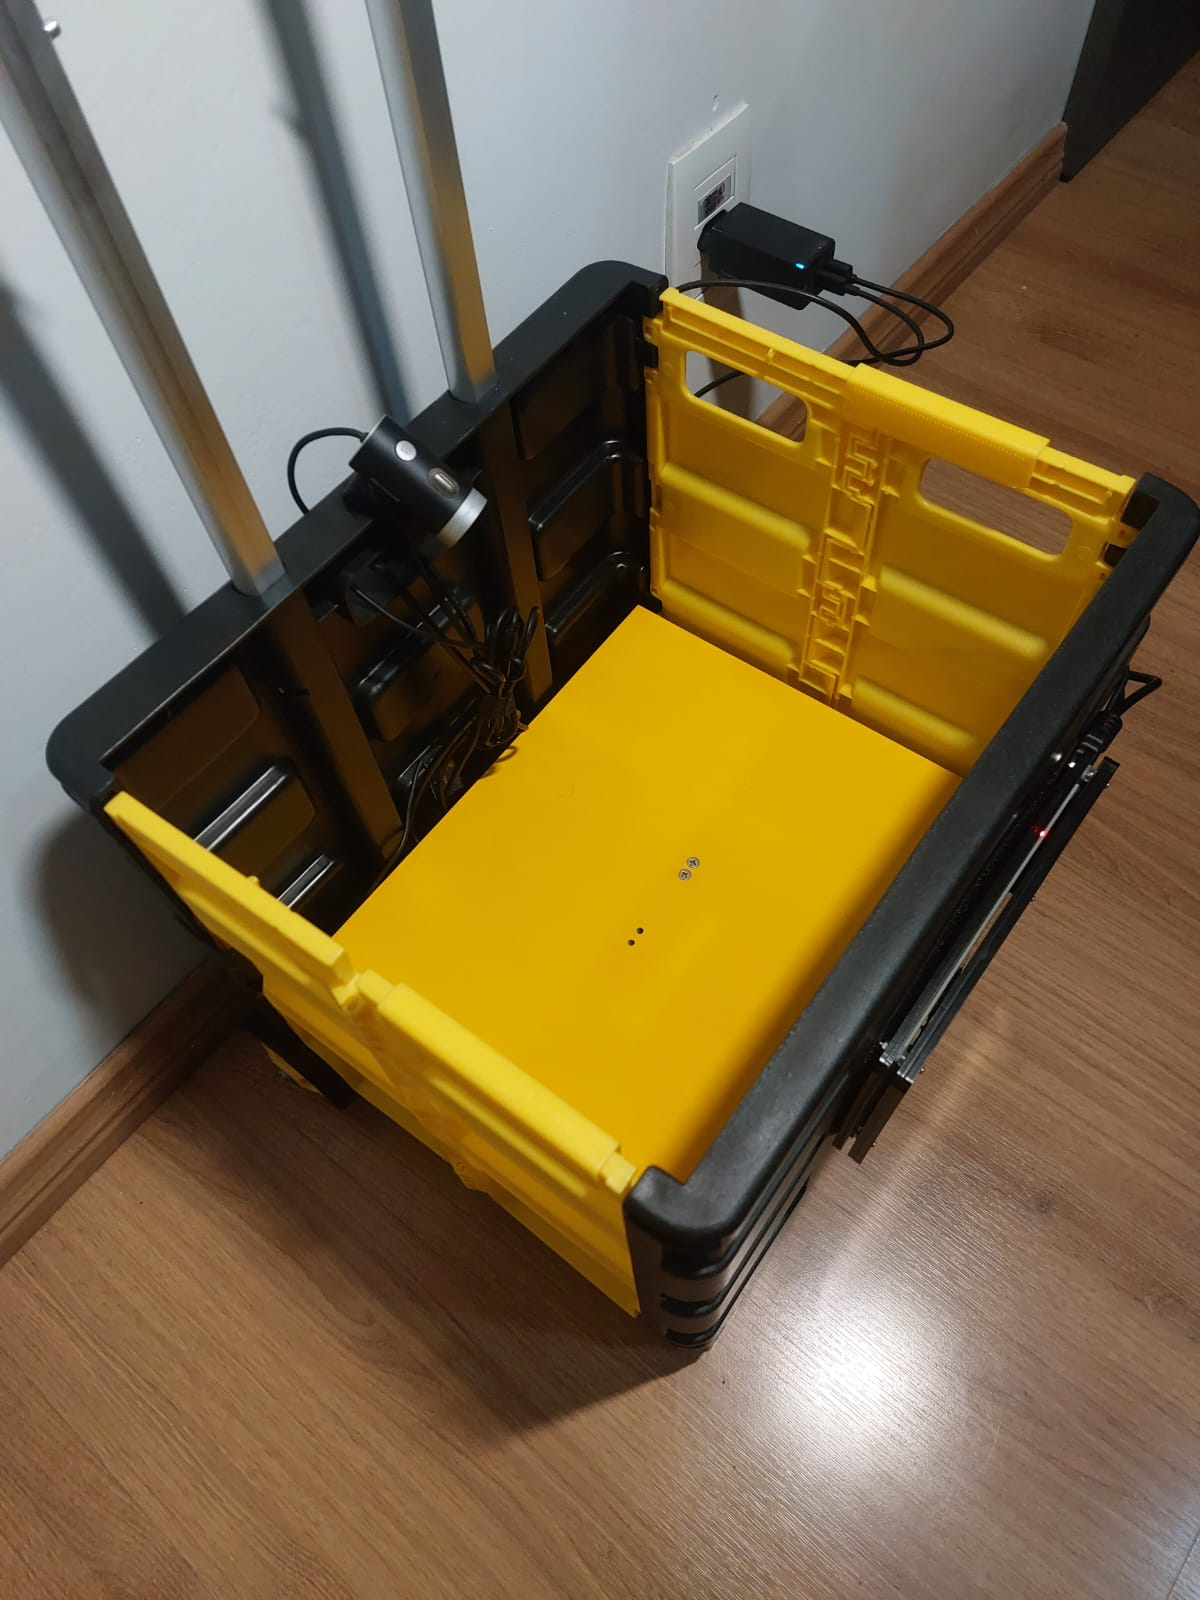
\includegraphics[width=0.5\textwidth]{./images/carttop.jpeg}
	\caption[Top view of the assembly showing the false bottom]{Top view of the assembly showing the false bottom}
	\fonte{Own work}
\end{figure}

Considering the objectives of the prototype, the shape of the mechanical
housing was not considered to be of great relevance and using a real
supermarket cart would have been impractical considering its size and cost. Still, we wanted
to keep a shape that would represent the overall idea of a smart cart.

\begin{figure}[H]
	\centering
	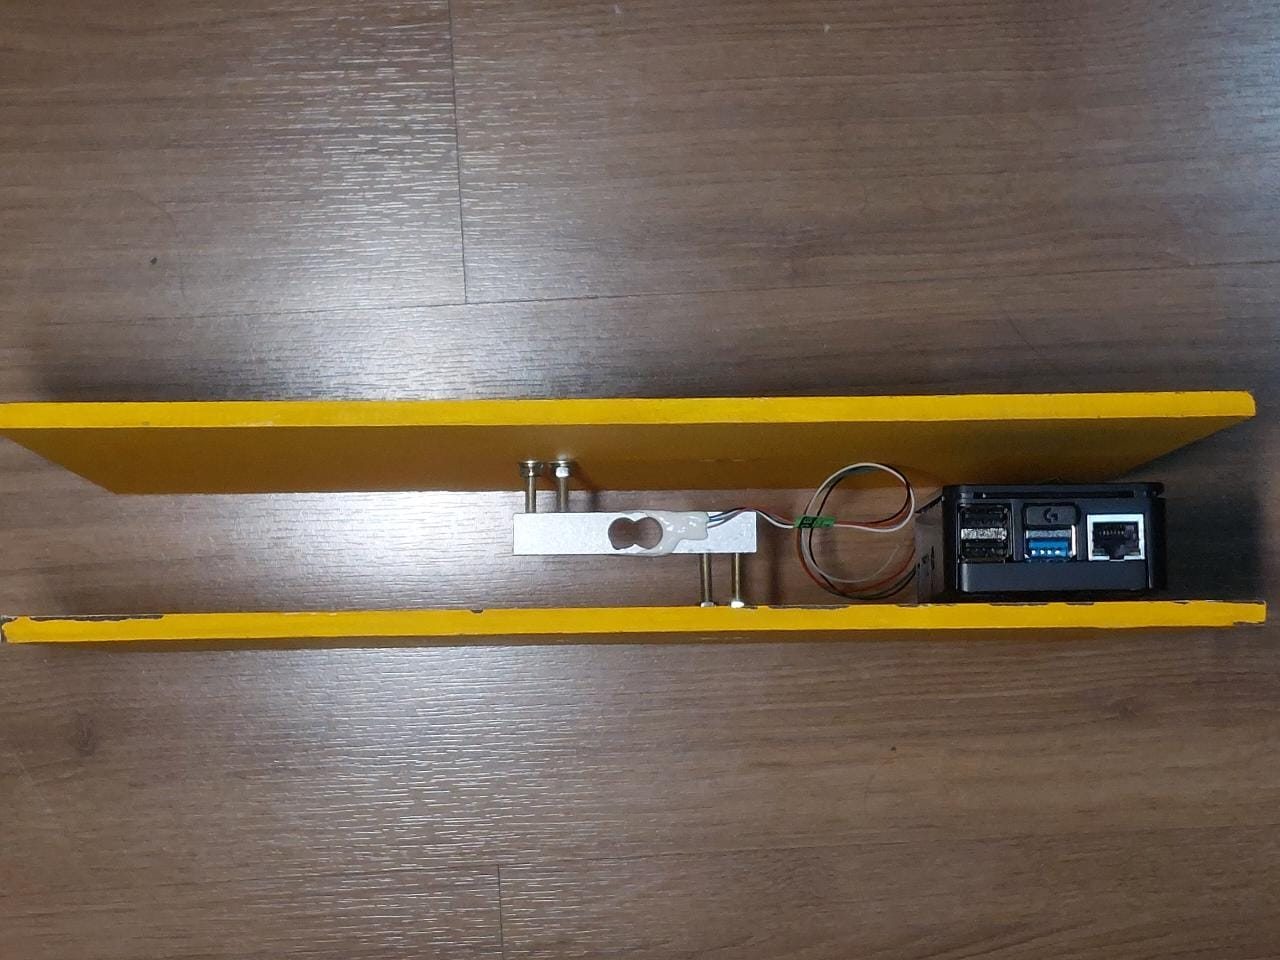
\includegraphics[width=0.6\textwidth]{./images/cartbase2.jpeg}
	\caption[False bottom structure with the load cell and Raspberry Pi board in between]{False bottom structure with the load cell and Raspberry Pi board in between}
	\fonte{Own work}
\end{figure}

Additional photos of the prototype can be seen on Appendix \ref{app:photos}.

\chapter{Results}

\section{Model Accuracy}

The most lightweight models were the preferred ones considering our edge device capabilities,
as they offer better inference time performance. 
However, we were also looking for the most optimal accuracy and loss metrics, 
therefore the models were evaluated with test images, which were never introduced to the models
during training, to make sure that they were efficient on the what they are ultimately supposed to do, 
which is to detect products.

Below you can find some examples of inferences executed in test images. 

\begin{figure}[H]
	\centering
	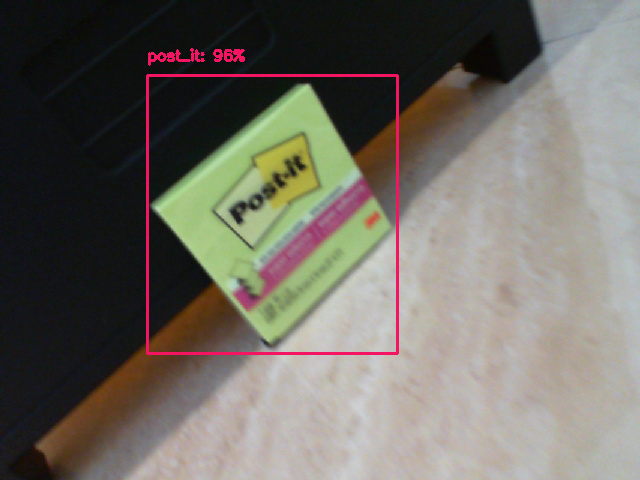
\includegraphics[width=0.5\textwidth]{./images/singlelabel-classification-1.png}
	\caption[Single-Label Classification Example 1]{Single-Label Classification Example 1}
	\fonte{Own work}
\end{figure}

\begin{figure}[H]
	\centering
	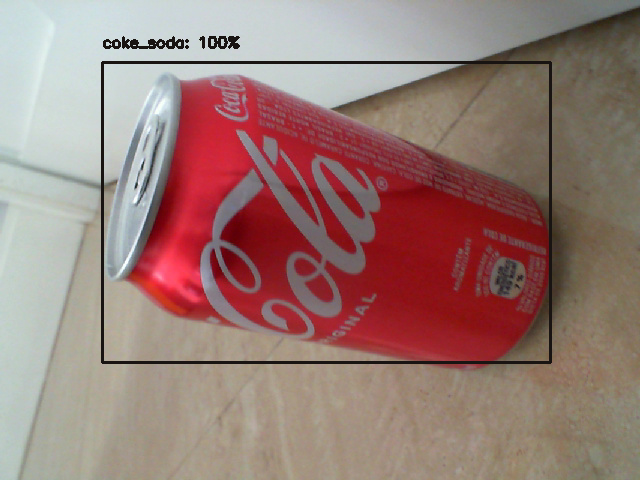
\includegraphics[width=0.5\textwidth]{./images/singlelabel-classification-2.png}
	\caption[Single-Label Classification Example 2]{Single-Label Classification Example 2}
	\fonte{Own work}
\end{figure}

\begin{figure}[H]
	\centering
	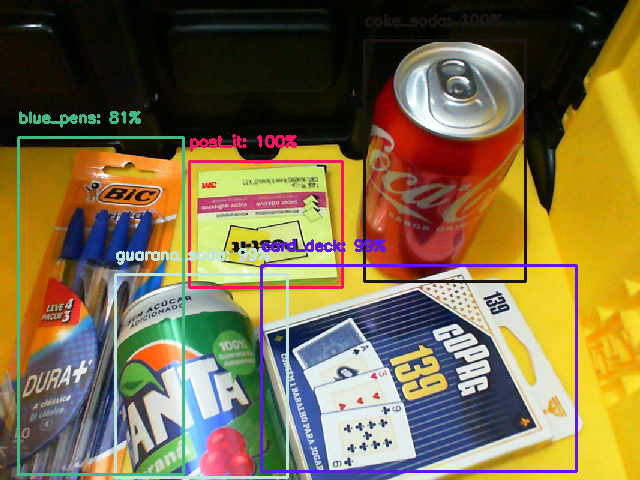
\includegraphics[width=0.5\textwidth]{./images/multilabel-classification-1.png}
	\caption[Multi-Label Classification Example 1]{Multi-Label Classification Example 1}
	\fonte{Own work}
\end{figure}

\begin{figure}[H]
	\centering
	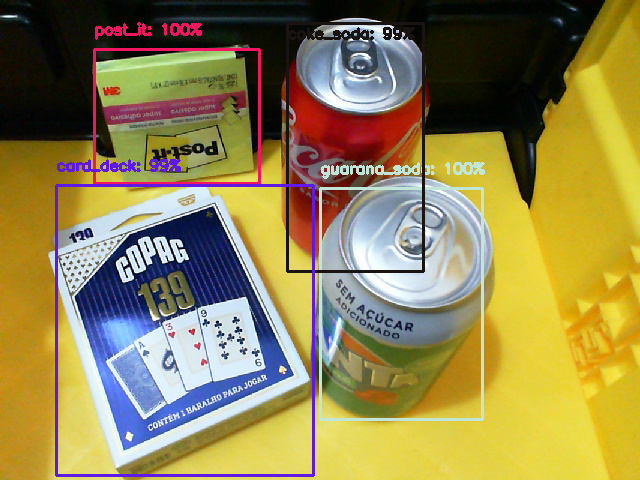
\includegraphics[width=0.5\textwidth]{./images/multilabel-classification-2.png}
	\caption[Multi-Label Classification Example 2]{Multi-Label Classification Example 2}
	\fonte{Own work}
\end{figure}

The accuracy metrics were also inferred in our Test data set by using the TensorFlow Lite's 
Object Detector \textit{"evaluate"} method\footnote{https://www.tensorflow.org/lite/api\_docs/python/tflite\_model\_maker/object\_detector/ObjectDetector\#evaluate}
for all different model configurations that were applied. 
The main evaluation metrics for the models considered for our product, which were the ones based 
in the EfficientDet-D0, D1 and D2 architectures- as the D3 and D4 architectures were too 
computationally expensive for our device- are listed below. 

\begin{table}[H]
	\centering
	\begin{adjustbox}{width=1\textwidth}
	\label{tab:modelPerformance}
	\begin{tabular}{c|c|c|c|c|c|c|c|c|c|c}
		\hline 
		Model Architecture & Preprocessing Strategy & Training Strategy & AP & AP 50 IoU & AP 75 IoU & AP (label 1) & AP (label 2) & AP (label 3) & AP (label 4) & AP (label 5) \\
		\hline
        Efficientdet\-D0 & Resizing & Transfer Learning & \texttt{0.537} & \texttt{0.704} & \texttt{0.650} & \texttt{0.541} & \texttt{0.495} & \texttt{0.675} & \texttt{0.525} & \texttt{0.447} \\
		Efficientdet\-D1 & Resizing & Transfer Learning & \texttt{0.633} & \texttt{0.794} & \texttt{ 0.776} & \texttt{0.439} & \texttt{0.671} & \texttt{0.807} & \texttt{0.631} & \texttt{0.619} \\
		Efficientdet\-D2 & Resizing & Transfer Learning & \texttt{0.670} & \texttt{0.798} & \texttt{0.776} & \texttt{0.676} & \texttt{0.590} & \texttt{0.838} & \texttt{0.567} & \texttt{0.684} \\
		Efficientdet\-D0 & Resizing & Whole & \texttt{0.777} & \texttt{0.912} & \texttt{0.867} & \texttt{0.577} & \texttt{0.724} & \texttt{0.891} & \texttt{0.913} & \texttt{0.779} \\
		Efficientdet\-D1 & Resizing & Whole & \texttt{0.815} & \texttt{0.945} & \texttt{0.896} & \texttt{0.658} & \texttt{0.794} & \texttt{0.890} & \texttt{0.975} & \texttt{0.757} \\
		Efficientdet\-D2 & Resizing & Whole & \texttt{0.820} & \texttt{0.928} & \texttt{0.878} & \texttt{0.630} & \texttt{0.784} & \texttt{0.905} & \texttt{1.000} & \texttt{0.782} \\
		Efficientdet\-D0 & Cropping & Transfer Learning & \texttt{0.463} & \texttt{0.632} & \texttt{0.577} & \texttt{0.371} & \texttt{0.413} & \texttt{0.626} & \texttt{0.465} & \texttt{0.440} \\
		Efficientdet\-D1 & Cropping & Transfer Learning & \texttt{0.515} & \texttt{0.659} & \texttt{0.594} & \texttt{0.376} & \texttt{0.532} & \texttt{0.741} & \texttt{0.486} & \texttt{0.440} \\
		Efficientdet\-D2 & Cropping & Transfer Learning & \texttt{0.505} & \texttt{0.684} & \texttt{0.617} & \texttt{0.442} & \texttt{0.604} & \texttt{0.554} & \texttt{0.345} & \texttt{0.580} \\
		Efficientdet\-D0 & Cropping & Whole & \texttt{0.817} & \texttt{0.905} & \texttt{0.897} & \texttt{0.804} & \texttt{0.862} & \texttt{0.620} & \texttt{0.969} & \texttt{0.831} \\
		Efficientdet\-D1 & Cropping & Whole & \texttt{0.805} & \texttt{0.926} & \texttt{0.903} & \texttt{0.800} & \texttt{0.761} & \texttt{0.687} & \texttt{0.950} & \texttt{0.829} \\
		Efficientdet\-D2 & Cropping & Whole & \texttt{0.803} & \texttt{0.930} & \texttt{0.912} & \texttt{0.799} & \texttt{0.814} & \texttt{0.657} & \texttt{0.913} & \texttt{0.832} \\
		\hline 
	\end{tabular}
	\end{adjustbox}
	\caption[Test Evaluation Metrics for the Different Strategies and Models Applied for Inference]{Test Evaluation Metrics for the Different Strategies and Models Applied for Inference}
	\fonte{Own work}
\end{table}

These numbers consist on the Average Precision (\sigla{AP}{Average Precision}), which provides us with 
a percentage that is directly proportional to the number of correctly labeled predictions
among the predictions made in the Test set; the AP considering an 
Intersection over Union(\sigla{IoU}{Intersection over Union}) of 50\%, which means that there is 
50\% of overlap between the predicted and the actual bounding boxes (this is measured by 
taking the area of the intersection of the two bounding boxes divided by the area of their union, 
hence the name); the AP considering an IoU of 75\%; and the individual APs for each label that 
we wanted to forecast. 

We could clearly see that, while the Transfer Learning models were much faster to train,
in our particular case, the Whole-trained models outperformed them. This could be 
due to the fact that our pictures and objects are different from the
ones that are present in the COCO-2017 dataset; or because a custom feature extractor- 
with custom hidden layer weights and biases- could have better performance with our pictures. 
In terms of the architectures, as expected, the D2 architecture offered more robust results, at least in
our models that applied resizing as a preprocessing strategy. We could not see much superior metrics for
the models that used cropping for the images preprocessing, and that might be because most of the 
bounding boxes ended up being cropped as well and, with that, we lost a portion of valuable label data. 

The loss (error) metrics during training were also computed for our Train and Validation sets during the 
200 epochs that were used for training our models using batches of 16 images, for all different 
settings that were employed to train them. We can clearly state that the model showed significant
improvement as the epochs progressed, and maybe more epochs would even have brought greater performance,
as the weights would have been even more fine-tuned. The trade-off, though, is that it would have 
taken more time and computer power to train the models.
Below you can find the Classification Loss chart for our three top models of choice, which were
the EfficientDet-D0, D1 and D2, whole-trained and that used resizing as a preprocessing strategy.

\begin{figure}[H]
	\centering
	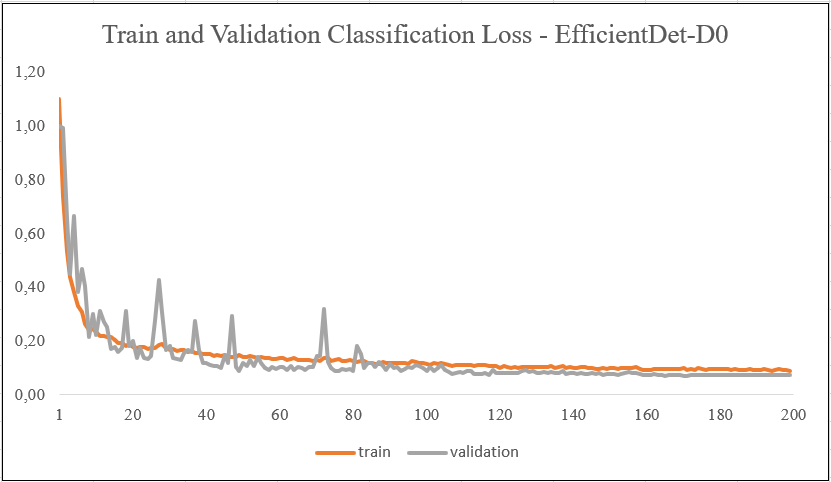
\includegraphics[width=0.65\textwidth]{./images/efficientdet-d0-resized-whole-loss.png}
	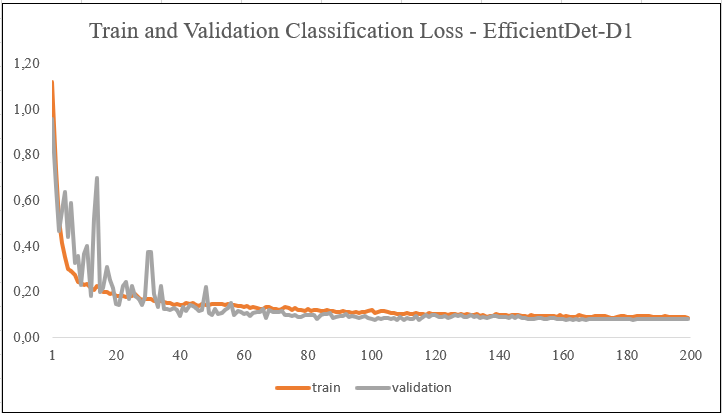
\includegraphics[width=0.65\textwidth]{./images/efficientdet-d1-resized-whole-loss.png}
	\includegraphics[width=0.65\textwidth]{./images/efficientdet-d2-resized-whole-loss.png}
	\caption[Train and Validation Classification Loss for the EfficientDet Models that 
		was whole-trained and took resized images as an input]{Train and Validation Classification Loss 
		for the EfficientDet Models that was whole-trained and took resized images as an input}
	\fonte{Own work}
\end{figure}

Note that those spikes in the loss values are probably due to the batch size, as it could be 
that in specific batches of 16 images the model was not fully prepared to predict the labels
in those images. Using a larger batch would likely solve it, however it would also take more RAM
memory consumption. 

Finally, to improve inference time performance, we also compiled our TensorFlow Lite models for 
usage with an Edge TPU, which further reduced our inference times. 

\begin{table}[H]
	\centering
	\begin{adjustbox}{width=1\textwidth}
	\label{tab:modelPerformance}
	\begin{tabular}{c|c|c|c|c}
		\hline 
		Model & FPS without the TPU & FPS using the TPU & CPU Ops using the TPU & TPU Ops using the TPU\\
		\hline
        Efficientdet-D0 Whole-Trained on Resized Images & \texttt{3.69} & \texttt{6.87} & \texttt{3} & \texttt{264}\\
		Efficientdet-D1 Whole-Trained on Resized Images & \texttt{2.09} & \texttt{5.14} & \texttt{131} & \texttt{191}\\
		Efficientdet-D2 Whole-Trained on Resized Images & \texttt{1.36} & \texttt{3.50} & \texttt{131} & \texttt{226}\\ 
		\hline 
	\end{tabular}
	\end{adjustbox}
	\caption[Inference Performance Metrics with and without the TPU]{Inference Performance Metrics with and without the TPU}
	\fonte{Own work}
\end{table}

\begin{figure}[H]
	\centering
	\includegraphics[width=0.5\textwidth]{./images/frameratemeasurement.png}
	\caption[Frame rate measurement]{Frame rate measurement}
\end{figure}

The inference speed has thoroughly improved, resulting in a greater capability to process more 
Frames Per Second. When we look at the number of CPU and TPU Operations, though, what we would
expect when using the TPU is that most Operations happen on the TPU side, however this behavior
could only be seen in the EfficientDet-D0 model. Part of it is because the EfficientDet-D0 model
has a simpler architecture, but it could also be due to the conversion of the model
for usage with the TPU or to the limited capacity of the TPU device that was used. For instance, Google
suggests using two TPU cores for the EfficientDet-D2 model\footnote{https://www.tensorflow.org/lite/models/modify/model\_maker/object\_detection}, 
because the tensors are too large to fit in the chip's memory.

Overall, after considering the tradeoff between precision and performance, we
have decided to use the EfficientDet-D2 model since its performance when paired
with the Coral TPU was more than enough for our purposes (around 4 FPS) and had
the best precision, improving the overall experience of the prototype.

\section{Power Consumption}

For estimating the overall power consumption, a commercial wattmeter was used
to observe the total power required by the power adapter used to supply energy
to the hardware components.

\begin{figure}[H]
	\centering
	\includegraphics[width=0.5\textwidth]{./images/powerconsumption.jpeg}
	\caption[Power consumption measurement using a wattmeter]{Power consumption measurement using a wattmeter}
	\fonte{Own work}
\end{figure}

During our tests, we have observed an average consumption of \textbf{10,4W}
when running the all the software and hardware components of the protype
through an external power adapter. 

The tests were performed on a 220V power line using the following equipment:
\begin{itemize}
    \item Sinotimer DDS108 Digital Wattmeter
    \item Baseus Quick Charger GaN 65W
\end{itemize}

Since both of these products do not have detailed accuracy and efficiency data
available, we estimate an overall 10\% margin of error considering their
construction \cite{Chen2017}. 

With that, we can assume that the actual power draw is between 9,4W and 11,4W.
Considering a desired  battery life of 24 hours, it would require a battery of
about 240 Wh, which can be found commercially and would not impose a
insurmountable practical barrier.

\section{Cost}

One of the important aspects when developing a marketable product is its \textbf{cost}.

A more detailed overview of the items and their costs in Brazil is shown on Table \ref{tbl:cost}.

\begin{table}[H]
	\centering
	\label{tab:correlacao}
	\begin{tabular}{c c c}
		\hline 
        Item & Quantity & Cost per item (BRL/USD) \\
		\hline
        Raspberry Pi 4 8GB Board &  1 & R\$ 1072,40 / US\$ 201,94 \\
        HX711 with breakout board &  1  & R\$ 2,55 / US\$ 0.48 \\
        10Kg Load Cell & 1 & R\$ 6,89 / US\$ 1,30 \\
        MDF Board &  2  & R\$ 10,00 / US\$ 1,89 \\
        Mounting hardware (screws, bolts and nuts) &  1  & R\$ 5,00 / US\$ 0,94 \\
        Foldable utility cart &  1  & R\$ 125,00 / US\$ 23,60 \\
        Webcam &  1  & R\$ 100,00 / US\$ 18.88 \\
		\hline 
        & Total cost & R\$ 1331.84 / US\$ 250.92 \\
        \hline
	\end{tabular}
    \caption[Items used on the prototype and their approximate retail cost in Brazil as of October 2022]{Items used on the prototype and their retail cost in October 2022}
	\fonte{Own work}
    \label{tbl:cost}
\end{table}

Of course, the developed prototype does not include all the necessary hardware
and software structure to deliver a successful product, but still it might show that at a
fundamental level, the cost of such a solution might not reach the costs that
current smart carts in the market sell for\footnote{The Nextop cart show on the
introduction currently retails for R\$ 120.000}.

Therefore, it might be possible to conclude that most of the retail cost of the
existing smart carts is not composed of the production and infrastructure costs
but from the required repayment of the research and development costs that such
a product demand.

\section{Challenges and future work}

As one of the expected outcomes of our work, we have been able to identify
several practical challenges that would need to be worked on for a marketable
product and will be discussed in the next sections.

\subsection{Extending the model for new products}
In a supermarket use case, we expect that products will need to be added or
removed from detection model on a regular basis. That becomes a challenge when
we consider the amount of data necessary to train the model used in the
developed prototype.

Considering that, an important next step on the development would be to work on
a model that can be easily extend to support new products without requiring too
much computational power for retraining.

\subsection{Deploying updates}

Considering the compute locality of the detection model used in the prototype,
which is the board embedded in the cart, deploying updates to the model to it
might become a challenge.

Changing the compute locality to  a Cloud infrastructure \cite{Aws2022} might
allow for easier deployment for updates but that comes with a trade off in
terms of latency, since networks calls would be required, and that can become
detrimental in such a real-time based product.

Investigating that trade off or even developing a solution for easy deployment
of model updates is another import development to be worked in the future. 

\subsection{Batteries and charging}

Another challenge identified for creating a viable product is to develop and
energy efficient solution that is capable of running on a reasonable battery
for at least an entire day.

As described in the testing section, the prototype is already capable of being
deployed with a reasonable commercial battery but we believe that there are
still margin for improvement.

Evidently, it is possible to include a battery with bigger capacity to the
product to provide better battery life but that comes with the trade off of
additional weight and cost, undesired characteristics from the end user and
grosser perspective respectively.

Additionally, it would be important to developed a practical mechanism to allow
the carts to be charged such as a docking mechanism or even by wireless
charging \cite{Treffers2015}, reducing the maintenance effort from the grocer
perspective. 

\subsection{Loss Prevention}

As our research has shown, loss prevention is a key feature of a smart cart, specially in the Brazilian context
\cite{Nextop2022}.

In such scenario, it would be important to work on possible extra features that
would give the grosser the extra confidence to deploy the cart to his/her retail
chain.

\subsection{Improving accuracy and reliability}

Related to the subsection above, improving the accuracy and reliability of the
overall system is key not just for loss prevention but to provide a great user
experience. We believe that a sub par experience will eventually lead to disuse
and therefore our objective would be to achieve a \textit{transparent}
experience, where the user might even forget about all the technological feat
that allows the cart to function.

\chapter{Conclusions}

This work has shown the development of \textit{zCart}, a functional smart cart
prototype using computer vision and sensor data, the same technological
framework used on similar commercial products. The prototype development has
successfully reached all of the desired objectives including the training of a
object detection model and developing an interactive user interface.

The real time performance achieved using the selected hardware was sufficient
for our purposes, at around 4 FPS with the EffiecientDet-D2 model, that showed an
average precision of about 80\% during validation.

Additionally, we were able to present some of the challenges and future work
discussions related to the current state of the prototype and also its cost
structure.


%---------- Referencias ----------
\clearpage
\label{bibstart}
\bibliography{reflatex}
\label{bibend}

%---------- Apendices (opcionais) ----------
\setcounter{chapter}{0}
\apendice
\chapter{User App screenshots}
\label{ap:userapp}

\begin{figure}[H]
	\centering
	\includegraphics[width=1\textwidth]{./images/userapp.png}
	\caption[]{Product listing and subtotal}
\end{figure}

\begin{figure}[H]
	\centering
	\includegraphics[width=1\textwidth]{./images/userapp2.png}
	\caption[]{Item addition notification}
\end{figure}

\begin{figure}[H]
	\centering
	\includegraphics[width=1\textwidth]{./images/userapp3.png}
	\includegraphics[width=1\textwidth]{./images/userapp3.png}
	\caption[]{Item removal notification}
\end{figure}

\begin{figure}[H]
	\centering
	\includegraphics[width=1\textwidth]{./images/userapp4.png}
	\caption[]{Pre-checkout confirmation popup}
\end{figure}

\begin{figure}[H]
	\centering
	\includegraphics[width=1\textwidth]{./images/userapp5.png}
	\caption[]{Post checkout screen}
\end{figure}

\apendice
\chapter{Prototype Photos}
\label{app:photos}

\begin{figure}[H]
	\centering
	\includegraphics[width=0.8\textwidth]{./images/20221204_164252.jpg}
	\caption[]{Frontal view of the prototype}
\end{figure}

\begin{figure}[H]
	\centering
    \includegraphics[width=0.8\textwidth]{./images/20221204_164147.jpg}
	\caption[]{Top view displaying the products in the cart}
\end{figure}

\begin{figure}[H]
	\centering
    \includegraphics[width=0.8\textwidth]{./images/20221204_163825.jpg}
	\caption[]{Frontal view of the prototype displaying the video camera feed}
\end{figure}

\begin{figure}[H]
	\centering
    \includegraphics[width=0.8\textwidth]{./images/20221204_164136.jpg}
	\caption[]{Frontal view of the prototype displaying the product listing}
\end{figure}

\begin{figure}[H]
	\centering
    \includegraphics[width=0.8\textwidth]{./images/20221204_161311.jpg}
    \caption[]{Popup confirmation before finishing the purchase}
\end{figure}

\begin{figure}[H]
	\centering
    \includegraphics[width=0.8\textwidth]{./images/20221204_161314.jpg}
	\caption[]{Checkout confirmation screen}
\end{figure}


\begin{figure}[H]
	\centering
    \includegraphics[width=0.7\textwidth]{./images/20221204_164249.jpg}
    \includegraphics[width=0.7\textwidth]{./images/20221204_164237.jpg}
	\caption[]{Product addition and removal notifications}
\end{figure}


\end{document}
